
\documentclass[xcolor=dvipsnames]{beamer}  % for hardcopy add 'trans'

\mode<presentation>
{
  \usetheme{Singapore}
  % or ...
  \setbeamercovered{transparent}
  % or whatever (possibly just delete it)
}

\usefonttheme{professionalfonts}
\usepackage[russian]{babel}
% or whatever
%\usepackage[latin1]{inputenc}
% or whatever
%\usepackage{times}
%\usepackage[T1]{fontenc}
% Or whatever. Note that the encoding and the font should match. If T1
% does not look nice, try deleting the line with the fontenc.

%%%%%%%%%%%%%%%%%%%%%% start my preamble %%%%%%%%%%%%%%%%%%%%%%


\addtobeamertemplate{navigation symbols}{}{%
    \usebeamerfont{footline}%
    \usebeamercolor[fg]{footline}%
    \hspace{1em}%
    \insertframenumber/\inserttotalframenumber
} 

\setbeamercolor{footline}{fg=blue}
\setbeamerfont{footline}{series=\bfseries}


%\usepackage{epsfig}
\usepackage{graphicx}
\graphicspath{{./figs_code/}}

\usepackage{amsmath, amssymb, amsthm}

\usepackage{fancyvrb}

\usepackage{tikz}
\usetikzlibrary{arrows}
\usetikzlibrary{calc}
\usetikzlibrary{intersections}
\usetikzlibrary{decorations}
\usepackage{pgf}
\usepackage{pgfplots}
\pgfplotsset{compat=1.13}

\usepackage{graphviz}
 
\usepackage{verbatim}


\usepackage{algorithmicx,algpseudocode}


%font
\usepackage{mathpazo}
%\usepackage[usenames, dvipsnames]{color}

%\usepackage[linesnumbered, ruled, lined]{algorithm2e}

\usepackage{xr}
\externaldocument[ET-]{et}


\newcommand*{\theorembreak}{\usebeamertemplate{theorem end}\framebreak\usebeamertemplate{theorem begin}}

\newcommand{\newtopic}[1]{\textcolor{Green}{\Large \bf #1}}
\newcommand{\navy}[1]{\textcolor{Blue}{\bf #1}}
\newcommand{\navymth}[1]{\textcolor{Blue}{#1}}
\newcommand{\red}[1]{\textcolor{red}{#1}}


\definecolor{pale}{RGB}{235, 235, 235}
\definecolor{pale2}{RGB}{175,238,238}
\definecolor{turquois4}{RGB}{0,134,139}

% Typesetting code
\definecolor{bg}{rgb}{0.95,0.95,0.95}
\usepackage{minted}
\usemintedstyle{friendly}
\newminted{python}{mathescape,frame=lines,framesep=4mm,bgcolor=bg}
\newminted{ipython}{mathescape,frame=lines,framesep=4mm,bgcolor=bg}
\newminted{julia}{mathescape,frame=lines,framesep=4mm,bgcolor=bg}
\newminted{c}{mathescape,linenos=true}
\newminted{r}{mathescape,  frame=none, baselinestretch=1, framesep=2mm}
\renewcommand{\theFancyVerbLine}{\sffamily
    \textcolor[rgb]{0.5,0.5,1.0}{\scriptsize {\arabic{FancyVerbLine}}}}


\usepackage{stmaryrd}

\newcommand{\Fact}{\textcolor{Brown}{\bf Факт. }}
\newcommand{\Facts}{\textcolor{Brown}{\bf Факты }}
\newcommand{\keya}{\textcolor{turquois4}{\bf Ключевая идея. }}
\newcommand{\Factnodot}{\textcolor{Brown}{\bf Факт }}
\newcommand{\Eg}{\textcolor{ForestGreen}{Пример. }}
\newcommand{\Egs}{\textcolor{ForestGreen}{Примеры. }}
\newcommand{\Ex}{{\bf Ex. }}
\newcommand{\Thm}{\textcolor{Brown}{\bf Теорема. }}
\newcommand{\Prf}{\textcolor{turquois4}{\bf Доказательство. }}
\newcommand{\Ass}{\textcolor{turquois4}{\bf Допущение.}} 
\newcommand{\Lem}{\textcolor{Brown}{\bf Лемма. }}

%source code 



% cali
\usepackage{mathrsfs}
\usepackage{bbm}
\usepackage{subfigure}

\newcommand{\argmax}{\operatornamewithlimits{argmax}}
\newcommand{\argmin}{\operatornamewithlimits{argmin}}

\newcommand\T{{\mathpalette\raiseT\intercal}}
\newcommand\raiseT[2]{\raisebox{0.25ex}{$#1#2$}}

\DeclareMathOperator{\cl}{cl}
%\DeclareMathOperator{\argmax}{argmax}
\DeclareMathOperator{\interior}{int}
\DeclareMathOperator{\Prob}{Prob}
\DeclareMathOperator{\kernel}{ker}
\DeclareMathOperator{\diag}{diag}
\DeclareMathOperator{\sgn}{sgn}
\DeclareMathOperator{\determinant}{det}
\DeclareMathOperator{\trace}{trace}
\DeclareMathOperator{\Span}{span}
\DeclareMathOperator{\rank}{rank}
\DeclareMathOperator{\cov}{cov}
\DeclareMathOperator{\corr}{corr}
\DeclareMathOperator{\range}{rng}
\DeclareMathOperator{\var}{var}
\DeclareMathOperator{\mse}{mse}
\DeclareMathOperator{\se}{se}
\DeclareMathOperator{\row}{row}
\DeclareMathOperator{\col}{col}
\DeclareMathOperator{\dimension}{dim}
\DeclareMathOperator{\fracpart}{frac}
\DeclareMathOperator{\proj}{proj}
\DeclareMathOperator{\colspace}{colspace}

\providecommand{\inner}[1]{\left\langle{#1}\right\rangle}

% mics short cuts and symbols
% mics short cuts and symbols
\newcommand{\st}{\ensuremath{\ \mathrm{s.t.}\ }}
\newcommand{\setntn}[2]{ \{ #1 : #2 \} }
\newcommand{\cf}[1]{ \lstinline|#1| }
\newcommand{\otms}[1]{ \leftidx{^\circ}{#1}}

\newcommand{\fore}{\therefore \quad}
\newcommand{\tod}{\stackrel { d } {\to} }
\newcommand{\tow}{\stackrel { w } {\to} }
\newcommand{\toprob}{\stackrel { p } {\to} }
\newcommand{\toms}{\stackrel { ms } {\to} }
\newcommand{\eqdist}{\stackrel {\textrm{ \scriptsize{d} }} {=} }
\newcommand{\iidsim}{\stackrel {\textrm{ {\sc iid }}} {\sim} }
\newcommand{\1}{\mathbbm 1}
\newcommand{\dee}{\,{\rm d}}
\newcommand{\given}{\, | \,}
\newcommand{\la}{\langle}
\newcommand{\ra}{\rangle}

\renewcommand{\rho}{\varrho}

\newcommand{\htau}{ \hat \tau }
\newcommand{\hgamma}{ \hat \gamma }

\newcommand{\boldx}{ {\mathbf x} }
\newcommand{\boldu}{ {\mathbf u} }
\newcommand{\boldv}{ {\mathbf v} }
\newcommand{\boldw}{ {\mathbf w} }
\newcommand{\boldy}{ {\mathbf y} }
\newcommand{\boldb}{ {\mathbf b} }
\newcommand{\bolda}{ {\mathbf a} }
\newcommand{\boldc}{ {\mathbf c} }
\newcommand{\boldi}{ {\mathbf i} }
\newcommand{\bolde}{ {\mathbf e} }
\newcommand{\boldp}{ {\mathbf p} }
\newcommand{\boldq}{ {\mathbf q} }
\newcommand{\bolds}{ {\mathbf s} }
\newcommand{\boldt}{ {\mathbf t} }
\newcommand{\boldz}{ {\mathbf z} }

\newcommand{\boldzero}{ {\mathbf 0} }
\newcommand{\boldone}{ {\mathbf 1} }

\newcommand{\boldalpha}{ {\boldsymbol \alpha} }
\newcommand{\boldbeta}{ {\boldsymbol \beta} }
\newcommand{\boldgamma}{ {\boldsymbol \gamma} }
\newcommand{\boldtheta}{ {\boldsymbol \theta} }
\newcommand{\boldxi}{ {\boldsymbol \xi} }
\newcommand{\boldtau}{ {\boldsymbol \tau} }
\newcommand{\boldepsilon}{ {\boldsymbol \epsilon} }
\newcommand{\boldmu}{ {\boldsymbol \mu} }
\newcommand{\boldSigma}{ {\boldsymbol \Sigma} }
\newcommand{\boldOmega}{ {\boldsymbol \Omega} }
\newcommand{\boldPhi}{ {\boldsymbol \Phi} }
\newcommand{\boldLambda}{ {\boldsymbol \Lambda} }
\newcommand{\boldphi}{ {\boldsymbol \phi} }

\newcommand{\Sigmax}{ {\boldsymbol \Sigma_{\boldx}}}
\newcommand{\Sigmau}{ {\boldsymbol \Sigma_{\boldu}}}
\newcommand{\Sigmaxinv}{ {\boldsymbol \Sigma_{\boldx}^{-1}}}
\newcommand{\Sigmav}{ {\boldsymbol \Sigma_{\boldv \boldv}}}

\newcommand{\hboldx}{ \hat {\mathbf x} }
\newcommand{\hboldy}{ \hat {\mathbf y} }
\newcommand{\hboldb}{ \hat {\mathbf b} }
\newcommand{\hboldu}{ \hat {\mathbf u} }
\newcommand{\hboldtheta}{ \hat {\boldsymbol \theta} }
\newcommand{\hboldtau}{ \hat {\boldsymbol \tau} }
\newcommand{\hboldmu}{ \hat {\boldsymbol \mu} }
\newcommand{\hboldbeta}{ \hat {\boldsymbol \beta} }
\newcommand{\hboldgamma}{ \hat {\boldsymbol \gamma} }
\newcommand{\hboldSigma}{ \hat {\boldsymbol \Sigma} }

\newcommand{\boldA}{\mathbf A}
\newcommand{\boldB}{\mathbf B}
\newcommand{\boldC}{\mathbf C}
\newcommand{\boldD}{\mathbf D}
\newcommand{\boldI}{\mathbf I}
\newcommand{\boldL}{\mathbf L}
\newcommand{\boldM}{\mathbf M}
\newcommand{\boldP}{\mathbf P}
\newcommand{\boldQ}{\mathbf Q}
\newcommand{\boldR}{\mathbf R}
\newcommand{\boldX}{\mathbf X}
\newcommand{\boldU}{\mathbf U}
\newcommand{\boldV}{\mathbf V}
\newcommand{\boldW}{\mathbf W}
\newcommand{\boldY}{\mathbf Y}
\newcommand{\boldZ}{\mathbf Z}

\newcommand{\bSigmaX}{ {\boldsymbol \Sigma_{\hboldbeta}} }
\newcommand{\hbSigmaX}{ \mathbf{\hat \Sigma_{\hboldbeta}} }

\newcommand{\RR}{\mathbbm R}
\newcommand{\CC}{\mathbbm C}
\newcommand{\NN}{\mathbbm N}
\newcommand{\PP}{\mathbbm P}
\newcommand{\EE}{\mathbbm E \nobreak\hspace{.1em}}
\newcommand{\EEP}{\mathbbm E_P \nobreak\hspace{.1em}}
\newcommand{\ZZ}{\mathbbm Z}
\newcommand{\QQ}{\mathbbm Q}


\newcommand{\XX}{\mathcal X}

\newcommand{\aA}{\mathcal A}
\newcommand{\fF}{\mathscr F}
\newcommand{\bB}{\mathscr B}
\newcommand{\iI}{\mathscr I}
\newcommand{\rR}{\mathscr R}
\newcommand{\dD}{\mathcal D}
\newcommand{\lL}{\mathcal L}
\newcommand{\llL}{\mathcal{H}_{\ell}}
\newcommand{\gG}{\mathcal G}
\newcommand{\hH}{\mathcal H}
\newcommand{\nN}{\textrm{\sc n}}
\newcommand{\lN}{\textrm{\sc ln}}
\newcommand{\pP}{\mathscr P}
\newcommand{\qQ}{\mathscr Q}
\newcommand{\xX}{\mathcal X}

\newcommand{\ddD}{\mathscr D}


\newcommand{\R}{{\texttt R}}
\newcommand{\risk}{\mathcal R}
\newcommand{\Remp}{R_{{\rm emp}}}

\newcommand*\diff{\mathop{}\!\mathrm{d}}
\newcommand{\ess}{ \textrm{{\sc ess}} }
\newcommand{\tss}{ \textrm{{\sc tss}} }
\newcommand{\rss}{ \textrm{{\sc rss}} }
\newcommand{\rssr}{ \textrm{{\sc rssr}} }
\newcommand{\ussr}{ \textrm{{\sc ussr}} }
\newcommand{\zdata}{\mathbf{z}_{\mathcal D}}
\newcommand{\Pdata}{P_{\mathcal D}}
\newcommand{\Pdatatheta}{P^{\mathcal D}_{\theta}}
\newcommand{\Zdata}{Z_{\mathcal D}}


\newcommand{\e}[1]{\mathbbm{E}[{#1}]}
\newcommand{\p}[1]{\mathbbm{P}({#1})}

%\theoremstyle{plain}
%\newtheorem{axiom}{Axiom}[section]
%\newtheorem{theorem}{Theorem}[section]
%\newtheorem{corollary}{Corollary}[section]
%\newtheorem{lemma}{Lemma}[section]
%\newtheorem{proposition}{Proposition}[section]
%
%\theoremstyle{definition}
%\newtheorem{definition}{Definition}[section]
%\newtheorem{example}{Example}[section]
%\newtheorem{remark}{Remark}[section]
%\newtheorem{notation}{Notation}[section]
%\newtheorem{assumption}{Assumption}[section]
%\newtheorem{condition}{Condition}[section]
%\newtheorem{exercise}{Ex.}[section]
%\newtheorem{fact}{Fact}[section]

% Bibliography
\usepackage[authordate,uniquename=false,firstinits,backend=biber,maxcitenames=2]{biblatex-chicago}
\DeclareFieldFormat[article]{title}{#1}
\DeclareFieldFormat[inproceedings]{title}{#1}
\addbibresource{et_newbib.bib}
\renewcommand{\cite}{\textcite}



\setlength{\parskip}{1.5ex plus0.5ex minus0.5ex}


\setlength{\jot}{12pt} 










\title{A Primer in Econometric Theory}

\subtitle
{Lecture 2: Linear Algebra and Matrices}

\author{John Stachurski \\ \tiny Lectures by Akshay Shanker}




\begin{document}

\begin{frame}
  \titlepage
\end{frame}

\section{Matrices and Linear Equations}

\begin{frame}
    
    \vspace{2em}
    \frametitle{Matrices}

    Typical \navy{$N \times K$ matrix}: 
    
    \begin{equation*}
        \boldA = 
        \left(
        \begin{array}{cccc}
            a_{11} & a_{12} & \cdots & a_{1K} \\
            a_{21} & a_{22} & \cdots & a_{2K} \\
            \vdots & \vdots &  & \vdots \\
            a_{N1} & a_{N2} & \cdots & a_{NK} 
        \end{array}
        \right)
    \end{equation*}
    %
    
    \vspace{.7em}
    Symbol $a_{nk}$ stands for element in the $n$-th row of the $k$-th column

\end{frame}


\begin{frame}
    
    \vspace{2em}
    $N \times K$ matrix also called a 
    %
    \begin{itemize}
        \item \navy{row vector} if $N = 1$
        \item \navy{column vector} if $K = 1$
    \end{itemize}
    
    \vspace{.7em}
    If $N = K$, then $\boldA$ is called \navy{square}
    
    If $\boldA$ is square and $a_{nk} = a_{kn}$ for every $k$ and $n$, then $\boldA$ is called \navy{symmetric}   
    
\end{frame}

\begin{frame}

    \vspace{2em}
    Often  elements of a matrix $\boldA$ represent coefficients in a system of linear
    equations
    %
    \begin{equation*}
        \label{eq:sleq}
        \begin{array}{c}
            a_{11} x_1 + a_{12} x_2 + \cdots + a_{1K} x_K = b_1 \\
            \vdots  \\
            a_{N1} x_1 + a_{N2} x_2 + \cdots + a_{NK} x_K = b_N 
        \end{array}
    \end{equation*}
    
\end{frame}

\begin{frame}

    \vspace{2em}
    For a matrix $\boldA$, the notation:
    \begin{itemize}
        \item $\row_n \boldA$ refers to the
    $n$th row of $\boldA$
        \item $\col_k \boldA$ to refers to the $k$th column of $\boldA$
    \end{itemize} 
    
    \vspace{.7em}
    The symbols $\boldzero$ and $\boldone$ represent matrices with all elements equal to zero and one respectively
    
\end{frame}

\begin{frame}
    
    \vspace{2em}
    For square $\boldA$, elements $a_{nn}$ called the \navy{principal diagonal}:
    %
    \begin{equation*}
        \left(
        \begin{array}{cccc}
            \red{a_{11}} & a_{12} & \cdots & a_{1N} \\
            a_{21} & \red{a_{22}} & \cdots & a_{2N} \\
            \vdots & \vdots &  & \vdots \\
            a_{N1} & a_{N2} & \cdots & \red{a_{NN}} \\
        \end{array}
        \right)
    \end{equation*}
    %

    \navy{Identity matrix}:
    %
    \begin{equation*}
        \boldI := 
        \left(
        \begin{array}{cccc}
            1 & 0 & \cdots & 0 \\
            0 & 1 & \cdots & 0 \\
            \vdots & \vdots &  & \vdots \\
            0 & 0 & \cdots & 1 \\
        \end{array}
        \right)
    \end{equation*}
    %
    Note  $\col_n \boldI = \bolde_n$, the $n$th canonical basis vector in $\RR^N$
    

\end{frame}

\begin{frame}
    \frametitle{Algebraic Operations for Matrices}

    \vspace{2em}
    Operations for matrices:
    
    \begin{itemize}
        \item Scalar multiplication 
        \item Addition
        \item Matrix multiplication
    \end{itemize}
    
    \vspace{.7em}
    Scalar multiplication is element by element, as with vectors:
    %
    \begin{equation*}
        \gamma 
        \left(
        \begin{array}{cccc}
            a_{11} & a_{12} & \cdots & a_{1K} \\
            a_{21} & a_{22} & \cdots & a_{2K} \\
            \vdots & \vdots &  & \vdots \\
            a_{N1} & a_{N2} & \cdots & a_{NK} \\
        \end{array}
        \right)
        :=
        \left(
        \begin{array}{cccc}
            \gamma a_{11} & \gamma a_{12} & \cdots & \gamma a_{1K} \\
            \gamma a_{21} & \gamma a_{22} & \cdots & \gamma a_{2K} \\
            \vdots & \vdots &  & \vdots \\
            \gamma a_{N1} & \gamma a_{N2} & \cdots & \gamma a_{NK} \\
        \end{array}
        \right)
    \end{equation*}
    %

\end{frame}

\begin{frame}
    
    \vspace{2em}
    Addition also element by element:
    %
    \begin{multline*}
        \left(
        \begin{array}{ccc}
            a_{11} & \cdots & a_{1K} \\
            a_{21} & \cdots & a_{2K} \\
            \vdots & \vdots & \vdots \\
            a_{N1} & \cdots & a_{NK} \\
        \end{array}
        \right)
        +
        \left(
        \begin{array}{ccc}
            b_{11} & \cdots & b_{1K} \\
            b_{21} & \cdots & b_{2K} \\
            \vdots & \vdots & \vdots \\
            b_{N1} & \cdots & b_{NK} \\
        \end{array}
        \right)
        \\
        :=
        \left(
        \begin{array}{ccc}
            a_{11} + b_{11} &  \cdots & a_{1K} + b_{1K} \\
            a_{21} + b_{21} &  \cdots & a_{2K} + b_{2K} \\
            \vdots & \vdots & \vdots \\
            a_{N1} + b_{N1} &  \cdots & a_{NK} + b_{NK} \\
        \end{array}
        \right)
    \end{multline*}
    %

    Note  matrices must be same dimension

\end{frame}

\begin{frame}
    
    \vspace{2em}
    Multiplication of matrices:  
    
    \vspace{.7em}
    Product $\boldA \boldB$: 
    $i,j$-th element is inner product of $i$-th row of $\boldA$ and 
    $j$-th column of $\boldB$  
    
    \begin{equation*}
    c_{ij} = \inner{\row_i \boldA,\,  \col_j  \boldB} = \sum_{k=1}^K a_{ik} b_{kj}
    \end{equation*}
    %
\end{frame}



\begin{frame}
    
    \vspace{2em}
    Picture for $i=j=1$:
    %
    \small\begin{equation*}
        \left(
        \begin{array}{ccc}
            \red{a_{11}} & \red{\cdots} & \red{a_{1K}} \\
            a_{21} & \cdots & a_{2K} \\
            \vdots & \vdots & \vdots \\
            a_{N1} & \cdots & a_{NK} \\
        \end{array}
        \right)
        \left(
        \begin{array}{ccc}
            \red{b_{11}} & \cdots & b_{1J} \\
            \red{b_{21}} & \cdots & b_{2J} \\
            \red{\vdots} & \vdots & \vdots \\
            \red{b_{K1}} & \cdots & b_{KJ} \\
        \end{array}
        \right)
        =
        \left(
        \begin{array}{ccc}
            \red{c_{11}} & \cdots & c_{1J} \\
            c_{21} & \cdots & c_{2J} \\
            \vdots & \vdots & \vdots \\
            c_{N1} & \cdots & c_{NJ} \\
        \end{array}
        \right)
    \end{equation*}
    
    \vspace{1em}
    In this picture, 
    %
    \begin{equation*}
        c_{11} = \inner{\row_1(\boldA) , \col_1 (\boldB)} = \sum_{k=1}^K a_{1k} b_{k1}
    \end{equation*}

\end{frame}

\begin{frame}
    
    \vspace{2em}
    Suppose $\boldA$ is $N \times K$ and $\boldB$ is $J \times M$
    
    \begin{itemize}
        \item $\boldA \boldB$ defined only if $K = J$
        \item Resulting matrix $\boldA \boldB$ is $N \times M$
    \end{itemize}
    
    \vspace{.7em}
    The rule to remember:
    %
    \begin{equation*}
        \text{product of } N \times K \text{ and } K \times M
        \text{ is }  N \times M
    \end{equation*}
    %

    Multiplication is not commutative: $\boldA \boldB \not= \boldB \boldA$ 
    
    Note $\boldB \boldA$ is not well-defined unless $N = M$ also holds 

\end{frame}


\begin{frame}
    
    \vspace{2em}
    \Fact{\eqref{ET-fa:bmari}}
        For conformable matrices $\boldA$, $\boldB$, $\boldC$ and scalar $\alpha$, we have
        %
        \begin{enumerate}
            \item $\boldA (\boldB \boldC) = (\boldA \boldB) \boldC$,
            \item $\boldA (\boldB + \boldC) = \boldA \boldB + \boldA \boldC$,
            \item $(\boldA + \boldB) \boldC = \boldA \boldC + \boldB \boldC$,
            \item $\boldA \alpha \boldB = \alpha \boldA \boldB$, and
            \item $\boldA \boldI = \boldA$ and $\boldI \boldA = \boldA$, where
                $\boldI$ is the identity matrix.
        \end{enumerate}
    
    Here, ``conformable'' means operation is defined given matrix dimensions

\end{frame}


\begin{frame}

    \vspace{2em}
    The \navy{$k$th power} of a square matrix $\boldA$ is defined as
    %    
    \begin{equation*}
        \boldA^k := \underbrace{\boldA \cdots \boldA}_{k \text{ terms}} 
    \end{equation*}
    
    \vspace{.7em}
    If $\boldB$ is such that $\boldB^2 = \boldA$, then $\boldB$
    is called the \navy{square root} of $\boldA$ and written $\sqrt{\boldA}$
    
\end{frame}

\begin{frame}

    \vspace{2em}
    Given $N \times K$ matrix $\boldA$ and $K \times 1$ column
    vector $\boldx$, the product $\boldA \boldx$ is:
    %
    \begin{align*}
        \boldA \boldx
        & = 
        \left(
        \begin{array}{cccc}
            a_{11} & a_{12} & \cdots & a_{1K} \\
            a_{21} & a_{22} & \cdots & a_{2K} \\
            \vdots & \vdots &  & \vdots \\
            a_{N1} & a_{N2} & \cdots & a_{NK} 
        \end{array}
        \right)
        \left(
        \begin{array}{c}
            x_1 \\
            x_2 \\
            \vdots \\
            x_K
        \end{array}
        \right)
        \\
        & =
        x_1 \left(
        \begin{array}{c}
            a_{11} \\
            a_{21} \\
            \vdots \\
            a_{N1} 
        \end{array}
        \right)
        +
        x_2 \left(
        \begin{array}{c}
            a_{12} \\
            a_{22} \\
            \vdots \\
            a_{N2} 
        \end{array}
        \right)
        + \cdots + 
        x_K \left(
        \begin{array}{c}
            a_{1K} \\
            a_{2K} \\
            \vdots \\
            a_{NK} 
        \end{array}
        \right)
        \\
        & = 
        \sum_{k=1}^K x_k \col_k \boldA
    \end{align*}
%
\end{frame}

\begin{frame}\frametitle{Matrices as Maps}

    \vspace{2em}
    We can think of an $N\times K$ matrix $\boldA$ as a map from
    $\mathbb{R}^{K}$ to $\mathbb{R}^{N}$:
    \[
        \boldx \mapsto \boldA\boldx 
    \]
    
    Such a map is linear
    
    \vspace{.7em}
    How about examples of linear functions that don't involve matrices? 
    
    ...actually, there are none! 
    
\end{frame}

\begin{frame}
    
    \vspace{.7em}
    The set of linear functions from $\RR^K$ to
    $\RR^N$ and the set of $N \times K$ matrices are in one-to-one correspondence:
    
    \vspace{.7em}
    \Thm{\eqref{ET-t:lmaeq}}
    Let $T$ be a function from $\RR^K$ to $\RR^N$. The following are
    equivalent:
    %
    \begin{enumerate}
        \item $T$ is linear.
        \item There exists an $N \times K$ matrix $\boldA$ such that $T\boldx
            = \boldA \boldx$ for all $\boldx \in \RR^K$.
    \end{enumerate}
    %
\end{frame}

\begin{frame}

    \vspace{2em}
    \Prf (1. $\implies$ 2.)
    
    Let $T \colon \RR^K \to \RR^N$ be linear
    
    We aim to construct an $N \times K$ matrix $\boldA$ such that
    %
    $$ T\boldx = \boldA \boldx, \qquad \forall \, \boldx \in \RR^K $$
    %
    As usual, let
    $\bolde_k$ be the $k$-th canonical basis vector in $\RR^K$
    
    Define a matrix $\boldA$ by $\col_k(\boldA) = T\bolde_k$. Pick any $\boldx = (x_1, \ldots, x_K) \in \RR^K$. By linearity we have,
    %
    \begin{equation*}
        T\boldx 
        = T \left[\sum_{k=1}^K x_k \bolde_k \right]
        = \sum_{k=1}^K x_k T \bolde_k
        = \sum_{k=1}^K x_k \col_k(\boldA)
        = \boldA \boldx
    \end{equation*}
    
\end{frame}

\begin{frame}
    
    \vspace{2em}
    \Prf (2 $\implies$ 1)
    %
    Fix $N \times K$ matrix $\boldA$ and let $T$ be defined by
    \begin{equation*}
        T \colon \RR^K \to \RR^N, 
        \qquad
        T\boldx = \boldA \boldx
    \end{equation*}

    Pick any $\boldx$, $\boldy$ in $\RR^K$, and any scalars $\alpha$ and $\beta$
     
    \vspace{.7em} 
    The rules of matrix arithmetic tell us that
    %
    \begin{equation*}
        T(\alpha \boldx + \beta \boldy) 
        := \boldA (\alpha \boldx + \beta \boldy)
        = \alpha \boldA \boldx  + \beta \boldA \boldy
        =: \alpha T\boldx + \beta T\boldy 
    \end{equation*}
    
\end{frame}

\begin{frame}
    
    \vspace{2em}
    Consider solving a system of linear equations such as
    $\boldA \boldx = \boldb$
    
    \vspace{.7em}
    Existence: can we find an $\boldx$ that satisfies this equation, for any
    given $\boldb$?  
    \begin{itemize}
        \item is the corresponding linear map $T\boldx = \boldA \boldx$ an onto function? 
        \item equivalently, is $\range T$ equal to all of $\RR^N$?
    \end{itemize}
    
\end{frame}


\begin{frame}\frametitle{Column Space}

    \vspace{2em}
    The range of $T$ is all vectors of the form
    $T\boldx = \boldA \boldx$ where $\boldx$ varies over $\RR^K$
    
    For $\boldx \in \RR^K$, we have
    \[\boldA \boldx = \sum_{k=1}^K x_k \col_k \boldA\]
    
    \vspace{.7em}
    Thus, $\range T$ equals the \navy{column space} of $\boldA$ -- the span of the columns of $\boldA$
    \begin{equation*}
    \label{eq:secolsp}
    \colspace \boldA := \Span \{ \col_1 \boldA, \ldots, \col_K \boldA \}
    \end{equation*}
    %
    In summary, 
    \begin{equation*}
        \colspace \boldA = \range T = \setntn{\boldA \boldx}{ \boldx \in \RR^K}
    \end{equation*}
    
\end{frame}


\begin{frame}
    \frametitle{Rank}

    \vspace{2em}
    Equivalent questions
    %
    \begin{itemize}
        \item How large is the range of the linear map $T \boldx = \boldA \boldx$?
        \item How large is the column space of $\boldA$?
    \end{itemize}

    \vspace{1em}

    The obvious measure of size for a linear subspace is its dimension
    
    The dimension of $\colspace \boldA$ is known as the \navy{rank} of $\boldA$  
    %
    \begin{equation*}
        \rank \boldA := \dim \colspace \boldA
    \end{equation*}
    %

    Because $\colspace \boldA$ is the span of $K$ vectors, we have
    %
    \begin{equation*}
        \rank \boldA = \dimension \colspace \boldA \leq K
    \end{equation*}


\end{frame}


\begin{frame}
    
    \vspace{2em}
    $\boldA$ has \navy{full column rank} if 
    %
    \begin{equation*}
        \rank \boldA = \text{ number of columns of } \boldA
    \end{equation*}

    \vspace{.7em}
    \Fact{\eqref{ET-fa:frie}} For any matrix $\boldA$,  the following statements are equivalent:
    %
    \begin{enumerate}
        \item $\boldA$ is of full column rank
            \vspace{0.3em} 
        \item The columns of $\boldA$ are linearly independent
            \vspace{0.3em} 
        \item If $\boldA \boldx = \boldzero$, then $\boldx = \boldzero$
    \end{enumerate}
    %

\end{frame}

\begin{frame}\frametitle{Square Matrices and Invertability}

    \vspace{2em}
    Consider the case where $\boldA$ is $N \times N$ 
   
   \vspace{.7em}
    We seek conditions on $\boldA$ under which, for every $\boldb \in \RR^N$, there
    exists exactly one $\boldx \in \RR^N$ such that $\boldA \boldx = \boldb$
    
    \vspace{.7em}
    Let $T$ be the linear map $T \boldx = \boldA \boldx$
    \begin{itemize}
        \item When
        does each point $\boldb \in \RR^N$ have one and only one preimage under $T$?
        \item Equivalenty, when is $T$ a bijection?
    \end{itemize}
    
\end{frame}

\begin{frame}
    
    \vspace{2em}
    Recall linear bijections are called nonsingular functions

    \vspace{.7em}
    \Fact{\eqref{ET-fa:exinv}}
        For $N \times N$ matrix $\boldA$, the following are equivalent:
        %
        \begin{enumerate}
            \item The columns of $\boldA$ are linearly independent.
            \item The columns of $\boldA$ form a basis of $\RR^N$.
            \item $\rank \boldA = N$.
            \item $\colspace \boldA = \RR^N$.
            \item $\boldA \boldx = \boldA \boldy \; \implies \; \boldx = \boldy$.
            \item $\boldA \boldx = \boldzero \; \implies \; \boldx = \boldzero$.
            \item For each $\boldb \in \RR^N$, the equation $\boldA \boldx = \boldb$
                has a solution.
            \item For each $\boldb \in \RR^N$, the equation $\boldA \boldx = \boldb$
                has a unique solution.
        \end{enumerate}

\end{frame}


\begin{frame}

    \vspace{2em}
    If any of the equivalent conditions in
    fact~\ref{ET-fa:exinv} are true we will call not just the map $T$ but also the
    underlying matrix $\boldA$ \navy{nonsingular}
    
    \vspace{.7em}
    If any one---and hence all---of
    these conditions fail, then $\boldA$ is called \navy{singular}
    
\end{frame}

\begin{frame}
    
    \vspace{2em}
    Any bijection has an inverse (see \S\ref{ET-ss:functions} in ET)
    
    \vspace{.7em}
    Any nonsingular map $T$ has a nonsingular inverse $T^{-1}$ (
    fact~\ref{ET-fa:nsins} on page~\pageref{ET-fa:nsins})
    
    \begin{itemize}
        \item where $T$ is generated by a matrix $\boldA$, the inverse $T^{-1}$ is also
        associated with a matrix, called the inverse of $\boldA$ 
    \end{itemize}

\end{frame}

\begin{frame}

    \vspace{2em}    
    \Thm{\eqref{ET-t:nonsigmat}}
        For nonsingular $\boldA$ the following statements are true:
        %
        \begin{enumerate}
            \item There exists a square matrix $\boldB$ such that $\boldA
                \boldB = \boldB \boldA = \boldI$, where $\boldI$ is the
                identity matrix.  The matrix $\boldB$ is called the \navy{inverse}
                of $\boldA$, and written as $\boldA^{-1}$.
            \item For each $\boldb \in \RR^N$, the unique solution to $\boldA \boldx =
                \boldb$ is given by 
                    %
                    \begin{equation*}
                        \label{eq:sofox}
                        \boldx = \boldA^{-1} \boldb
                    \end{equation*}
                    %
        \end{enumerate}

\end{frame}

\begin{frame}
    
    \vspace{2em}
    \Eg
    Consider the $N$ good linear demand system
    %
    \begin{equation*}
        q_n = \sum_{k=1}^N a_{nk} p_k + b_n,
        \quad n = 1, \ldots, N
    \end{equation*}
    %
    where $q_n$ and $p_n$ are quantity and price of the $n$th good
    
    \vspace{.7em}
    We want to compute the inverse demand function which gives prices in terms of quantities
    
    \vspace{.7em}
    Write the system
    in matrix form as $\boldq = \boldA \boldp + \boldb$
    
    If the columns of $\boldA$ are linearly independent, then 
    we can invert the system-- a unique solution
    exists for each fixed $\boldq$ and $\boldb$:
    %
    \[\boldp = \boldA^{-1} (\boldq - \boldb)\]
    
\end{frame}

\begin{frame}

    \vspace{.7em}    
    For $N\times N$ matrices $\boldA$ and $\boldB$, if
    
    \begin{itemize}
        \item $\boldB$ is a
        \navy{left inverse}, that is, $\boldB \boldA = \boldI$ 
        \item  or $\boldB$ is a\navy{right inverse}, that is, $\boldA \boldB = \boldI$ 
    \end{itemize}

    \vspace{.7em}    
    Then $\boldA$ is invertible and $\boldB$ is the inverse of $\boldA$
    
    \vspace{.7em}
    \Fact{\eqref{ET-fa:lrinv}}
    Let $\boldA$ and $\boldB$ be $N \times N$ square matrices.
    If $\boldB$ is either a left or a right inverse of $\boldA$,
    then $\boldA$ is nonsingular and $\boldB$ is its inverse.
 

\end{frame}

\begin{frame}

    \vspace{.7em}
    \Fact{\eqref{ET-fa:bpiv}}
    If $\boldA$ and $\boldB$ are nonsingular and $\alpha \not= 0$, then
    %
    \begin{enumerate}
        \item $(\boldA^{-1})^{-1} = \boldA$,
        \item $(\alpha \boldA)^{-1} = \alpha^{-1} \boldA^{-1}$, and 
        \item $(\boldA \boldB)^{-1} = \boldB^{-1} \boldA^{-1}$
    \end{enumerate}
    
\end{frame}

\begin{frame}\frametitle{Determinants}

    \vspace{.7em}
    Determinant is a unique number for each square matrix $\boldA$
    
    Let $S(N)$ be
    the set of all bijections from $\{1, \ldots, N\}$ to itself
    
    \vspace{.7em}
    For $\pi \in S(N)$, define the \navy{signature} of $\pi$ 
    %
    \begin{equation*}
        \sgn(\pi) := \prod_{m < n} \frac{\pi(m) - \pi(n)}{m - n}
    \end{equation*}
    
    \vspace{1em}
    The \navy{determinant} of $N \times N$ matrix $\boldA$ is
    
    \begin{equation*}
        \det \boldA 
        := \sum_{\pi \in S(N)} \sgn(\pi) \prod_{n=1}^N a_{\pi(n) n}
    \end{equation*}
    
\end{frame}

\begin{frame}

    \vspace{.7em}
    \Fact
    \eqref{ET-fa:detfacts}
    If $\boldI$ is the $N \times N$ identity, $\boldA$ and $\boldB$ are $N
    \times N$ matrices and $\alpha \in \RR$, then
    %
    \begin{enumerate}
        \item $\det \boldI = 1$,
        \item $\boldA$ is nonsingular if and only if $\det \boldA
            \not= 0$,
        \item $\det(\boldA\boldB) = \det(\boldA)
            \det(\boldB)$,
        \item $\det(\alpha \boldA) = \alpha^N \det(\boldA)$, and
        \item $\det(\boldA^{-1}) = (\det(\boldA))^{-1}$.
    \end{enumerate}
    
    \vspace{.7em}
    In the $2 \times 2$ case one can show that the determinant satisfies
    %
    \begin{equation*}
        \label{eq:det22}
        \det 
        \left(
        \begin{array}{cc}
            a & b  \\
            c & d  \\
        \end{array}
        \right)
        = ad - bc
    \end{equation*}
    
\end{frame}


\begin{frame}

    \vspace{2em}
    \Prf (Fact \ref{ET-fa:lrinv})
    
    Fix square matrix $\boldA$ and suppose a right
    inverse $\boldB$ exists: \[\boldA \boldB = \boldI\]
    
    Then both $\boldA$ and $\boldB$ are nonsingular,  since using the rules
    in fact~\ref{ET-fa:detfacts}: \[\det(\boldA) \det(\boldB) = 1\]
    
    Both $\det \boldA$ and $\det \boldB$ are nonzero and hence both
    matrices are nonsingular. Next, $\boldA \boldB = \boldI$, hence 
    %
    \[\boldB \boldA \boldB = \boldB\]
    %
    Post-multiplying by $\boldB^{-1}$ gives $\boldB \boldA = \boldI$
    
\end{frame}

\section{Properties of Matrices}

\begin{frame}\frametitle{Diagonal and Triangular Matrices}
    
    \vspace{2em}
    A square matrix is called \navy{lower triangular} if every element strictly above the
    principle diagonal is zero
    
    \vspace{.7em}
    \Eg
    %
    \begin{equation*}
        \label{eq:ltute}
        \boldL :=
        \left(
        \begin{array}{ccc}
            1 & 0 & 0  \\
            2 & 5 & 0 \\
            3 & 6 & 1
        \end{array}
        \right)
    \end{equation*}
    
\end{frame}

\begin{frame}

    \vspace{2em}
    A square matrix is called \navy{upper triangular} if every element
    strictly below the principle diagonal is zero

    \vspace{.7em}
    \Eg
    %
    \begin{equation*}
        \boldU :=
        \left(
        \begin{array}{ccc}
            1 & 2 & 3  \\
            0 & 5 & 6 \\
            0 & 0 & 1
        \end{array}
        \right)
    \end{equation*}
    
    \vspace{.7em}
    A square matrix is called \navy{triangular} if it is either upper or lower triangular

    \vspace{.7em}
    \Fact\eqref{ET-fa:dtmat}
    If $\boldA = (a_{mn})$ is triangular, then $\det \boldA = \prod_{n=1}^N a_{nn}$.
    
\end{frame}

\begin{frame}

    \vspace{2em}
    Associated linear equations also simple to solve 

  \vspace{0.7em}

    \Eg
    % 
    \begin{equation*}
        \left(
        \begin{array}{ccc}
            1 & 0 & 0  \\
            2 & 5 & 0 \\
            3 & 6 & 1
        \end{array}
        \right)
        \left(
        \begin{array}{ccc}
            x_1 \\
            x_2 \\
            x_3 
        \end{array}
        \right)
        =
        \left(
        \begin{array}{c}
            b_1 \\
            b_2 \\
            b_3 \\
        \end{array}
        \right)
    \end{equation*}
    
    becomes

    \begin{equation*}
        \begin{array}{c}
            x_1  = b_1  \\
            2x_1 + 5x_2 = b_2 \\
            3x_1 + 6x_2 + x_3 = b_3
        \end{array}
    \end{equation*}
    %

    Top equation involves only $x_1$, so can solve for it directly

    Plug that value into second equation, solve out for $x_2$, etc.

\end{frame}


\begin{frame}

    \vspace{2em}
    Consider a square $N \times N$ matrix $\boldA$

    \vspace{1em}

    The $N$ elements of the form $a_{nn}$ are called the \navy{principal diagonal}

    \vspace{1em}
    \begin{equation*}
        \left(
        \begin{array}{cccc}
            \red{a_{11}} & a_{12} & \cdots & a_{1N} \\
            a_{21} & \red{a_{22}} & \cdots & a_{2N} \\
            \vdots & \vdots &  & \vdots \\
            a_{N1} & a_{N2} & \cdots & \red{a_{NN}} \\
        \end{array}
        \right)
    \end{equation*}
    %

\end{frame}


\begin{frame}
    
    \vspace{2em}
    A square matrix $\boldD$ is called \navy{diagonal} if all entries off the
    principal diagonal are zero

    \begin{equation*}
        \boldD = 
        \left(
        \begin{array}{cccc}
            d_1 & 0 & \cdots & 0 \\
            0 & d_2 & \cdots & 0 \\
            \vdots & \vdots &  & \vdots \\
            0 & 0 & \cdots & d_N \\
        \end{array}
        \right)
    \end{equation*}

    \vspace{1em}

    Often written as
    
    \begin{equation*}
        \boldD = \diag(d_1, \ldots, d_N) 
    \end{equation*}

\end{frame}



\begin{frame}
    
    \vspace{2em}
    Diagonal systems are very easy to solve

    \vspace{0.5em}

    \Eg

    \begin{equation*}
        \begin{pmatrix}
            d_1 & 0  & 0 \\
            0 & d_2 & 0 \\
            0 & 0 & d_3 
        \end{pmatrix}
        \begin{pmatrix}
            x_1  \\
            x_2  \\
            x_3 
        \end{pmatrix}
        =
        \begin{pmatrix}
            b_1  \\
            b_2  \\
            b_3 
        \end{pmatrix}
    \end{equation*}

    is equivalent to

    \begin{equation*}
        \begin{array}{c}
            d_1 x_1  = b_1  \\
            d_2x_2 = b_2 \\
            d_3 x_3 = b_3
        \end{array}
    \end{equation*}

\end{frame}

\begin{frame}
    
    \vspace{2em}
    \Fact\eqref{ET-fa:powdm} If $\boldC = \diag(c_1, \ldots, c_N)$ and $\boldD = \diag(d_1, \ldots,
    d_N)$, then
    %
    \begin{enumerate}
        \item $\boldC + \boldD = \diag(c_1 + d_1, \ldots, c_N + d_N)$
            \vspace{0.4em}
        \item $\boldC \boldD = \diag(c_1 d_1, \ldots, c_N d_N)$
            \vspace{0.4em}
        \item $\boldD^k = \diag(d^k_1, \ldots, d^k_N)$ for any $k \in \NN$
            \vspace{0.4em}
        \item $d_n \geq 0$ for all $n$ $\implies$ $\boldD^{1/2}$ exists and equals
            %
            $$\diag(\sqrt{d_1}, \ldots, \sqrt{d_N})$$
            \vspace{-1.5em}
        \item $d_n \not= 0$ for all $n$ $\implies$ $\boldD$ is nonsingular and 
            %
            $$\boldD^{-1} = \diag(d_1^{-1}, \ldots, d_N^{-1})$$
    \end{enumerate}
    %

    \vspace{1em}

    Proofs: Check 1 and 2 directly. Parts 3-5 then follow from 1 and 2. 

\end{frame}


\begin{frame}\frametitle{Trace, Transpose, Symmetry}
    
    The \navy{trace} of a square matrix is defined by 
    %
    \vspace{0.5em}
    \begin{equation*}
        \trace \left(
        \begin{array}{ccc}
            a_{11} &  \cdots & a_{1N} \\
            \vdots & &  \vdots \\
            a_{N1} &  \cdots & a_{NN} \\
        \end{array}
        \right)
        = 
        \sum_{n=1}^N a_{nn}
    \end{equation*}
    %

    \vspace{0.5em}

    \vspace{0.5em}

    \Fact{\eqref{ET-fa:lmpt}} If $\boldA$ and $\boldB$ are square matrices and
    $\alpha, \beta \in \RR$, then 
    %
    \begin{equation*}
        \trace(\alpha \boldA + \beta \boldB) 
        = \alpha \trace(\boldA) + \beta \trace(\boldB)
    \end{equation*}
    %

    \vspace{0.5em}
    If 
    $\boldA$ is $N \times M$ and $\boldB$ is $M \times N$, then 
    $\trace(\boldA \boldB) = \trace(\boldB \boldA)$

\end{frame}

\begin{frame}
    
    \vspace{2em}
    The \navy{transpose} of $N \times K$ matrix $\boldA$ is a $K
    \times N$ matrix $\boldA^\T$ defined by 
    $$\col_n(\boldA') = \row_n(\boldA)$$

    \Eg If
    %
    \begin{equation*}
        \label{eq:aandb}
        \boldA := 
        \left(
        \begin{array}{cc}
            10 & 40  \\
            20 & 50  \\
            30 & 60
        \end{array}
        \right)
        \quad \text{then} \quad
        \boldA' = 
        \left(
        \begin{array}{ccc}
            10 & 20 & 30 \\
            40 & 50 & 60 
        \end{array}
        \right)
    \end{equation*}
    %

    If
    %
    \begin{equation*}
        \boldB := 
        \left(
        \begin{array}{ccc}
            1 & 3 & 5 \\
            2 & 4 & 6 \\
        \end{array}
        \right)
        \quad \text{then} \quad
        \boldB' := 
        \left(
        \begin{array}{cc}
            1 & 2  \\
            3 & 4  \\
            5 & 6 
        \end{array}
        \right)
    \end{equation*}
    %

\end{frame}

\begin{frame}

    \vspace{2em}
    A square matrix $\boldA$ is called \navy{symmetric} if $\boldA^\T = \boldA$
    \begin{itemize}
        \item equivalently, $a_{nk} = a_{kn}$ for every $k$ and $n$
    \end{itemize}
    
    \vspace{.7em}
    The matricies $\boldA^\T
    \boldA$ and $\boldA \boldA^\T$ are always well-defined and symmetric
    
\end{frame}

\begin{frame}
    
    \vspace{2em}
    \Fact{\eqref{ET-fa:owtra}}
    For conformable matrices $\boldA$ and $\boldB$, transposition satisfies
    %
    \begin{enumerate}
        \item $(\boldA^\T)^\T = \boldA$,
        \item $(\boldA \boldB)^\T = \boldB^\T \boldA^\T$,
        \item $(\boldA + \boldB)^\T = \boldA^\T +  \boldB^\T$, and
        \item $(c \boldA)^\T = c \boldA^\T$ for any constant $c$.
    \end{enumerate}

\end{frame}

\begin{frame}

    \vspace{2em}
    \Fact{\eqref{ET-fa:owtra2}}
        For each square matrix $\boldA$, we have 
        %
        \begin{enumerate}
            \item $\trace(\boldA) = \trace(\boldA^\T)$ and
            \item $\det(\boldA^\T) = \det(\boldA)$.
            \item If $\boldA$ is nonsingular, then so is $\boldA^\T$, and
                its inverse is $(\boldA^\T)^{-1}= (\boldA^{-1})^\T$.
        \end{enumerate}
        
    \vspace{.7em}
    If $\bolda$ and $\boldb$ are $N \times 1$ vectors, then the matrix
    product $\bolda^\T \boldb = \boldb^\T \bolda$ is equal to $\sum_{n=1}^N a_n b_n$,
    
    \begin{itemize}
        \item same as the inner product $\inner{\bolda, \boldb}$
    \end{itemize}

\end{frame}


\begin{frame}

    \frametitle{Eigenvalues and Eigenvectors}

    \vspace{2em}
    Let $\boldA$ be $N \times N$  
    
    In general $\boldA$ maps $\boldx$ to some arbitrary new location $\boldA \boldx$

    But sometimes $\boldx$ will only be \underline{scaled}:
    %
    \begin{equation}
        \label{eq:eiei}
        \boldA \boldx = \lambda \boldx
        \quad \text{for some scalar $\lambda$}
    \end{equation}
    
    \vspace{.7em}
    If \eqref{eq:eiei} holds and $\boldx$ is nonzero, then 
    %
    \begin{enumerate}
        \item $\boldx$ is called an \navy{eigenvector} of $\boldA$
            and $\lambda$ is called an \navy{eigenvalue}
            \vspace{0.3em}
        \item $(\boldx, \lambda)$ is called an \navy{eigenpair}
    \end{enumerate}

    Clearly $(\boldx, \lambda)$ is an eigenpair of $\boldA$ $\implies$
    $(\alpha \boldx, \lambda)$ is an eigenpair 
    of $\boldA$ for any nonzero $\alpha$

\end{frame}

\begin{frame}
    
    \vspace{2em}
    \Eg Let
    %
    $$
    \boldA :=
    \begin{pmatrix}
        1 & -1 \\
        3 & 5
    \end{pmatrix}
    $$

    Then
    
    $$
    \lambda = 2 
    \quad \text{ and } \quad
    \boldx
    =
    \begin{pmatrix}
        1 \\
        -1
    \end{pmatrix}
    $$

    form an eigenpair because $\boldx \not= \boldzero$ and

    $$
    \boldA \boldx =
    \begin{pmatrix}
        1 & -1 \\
        3 & 5
    \end{pmatrix}
    \begin{pmatrix}
        1 \\
        -1
    \end{pmatrix}
    =
    \begin{pmatrix}
        2 \\
        -2
    \end{pmatrix}
    = 2
    \begin{pmatrix}
        1 \\
        -1
    \end{pmatrix}
    =
    \lambda \boldx 
    $$

\end{frame}

\begin{frame}
    
    \vspace{2em}
    \Eg Consider the matrix 
    %
    \begin{equation*}
        \boldR := 
        \left(
        \begin{array}{cc}
            0 & -1  \\
            1 & 0  \\
        \end{array}
        \right)
    \end{equation*}
    %

    Induces counter-clockwise rotation on any point by $90^{\circ}$

    Hence no point $\boldx$ is scaled
    
    Hence there exists \underline{no} pair $\lambda \in \RR$ and $\boldx \not=
    \boldzero$
    such that
    %
    $$\boldR \boldx = \lambda \boldx$$  
    %
    
    \begin{itemize}
        \item In other words, no \underline{real-valued} eigenpairs exist
    \end{itemize}


\end{frame}

\begin{frame}
    
    \vspace{2em}
    \begin{figure}
       \begin{center}
        \scalebox{.4}{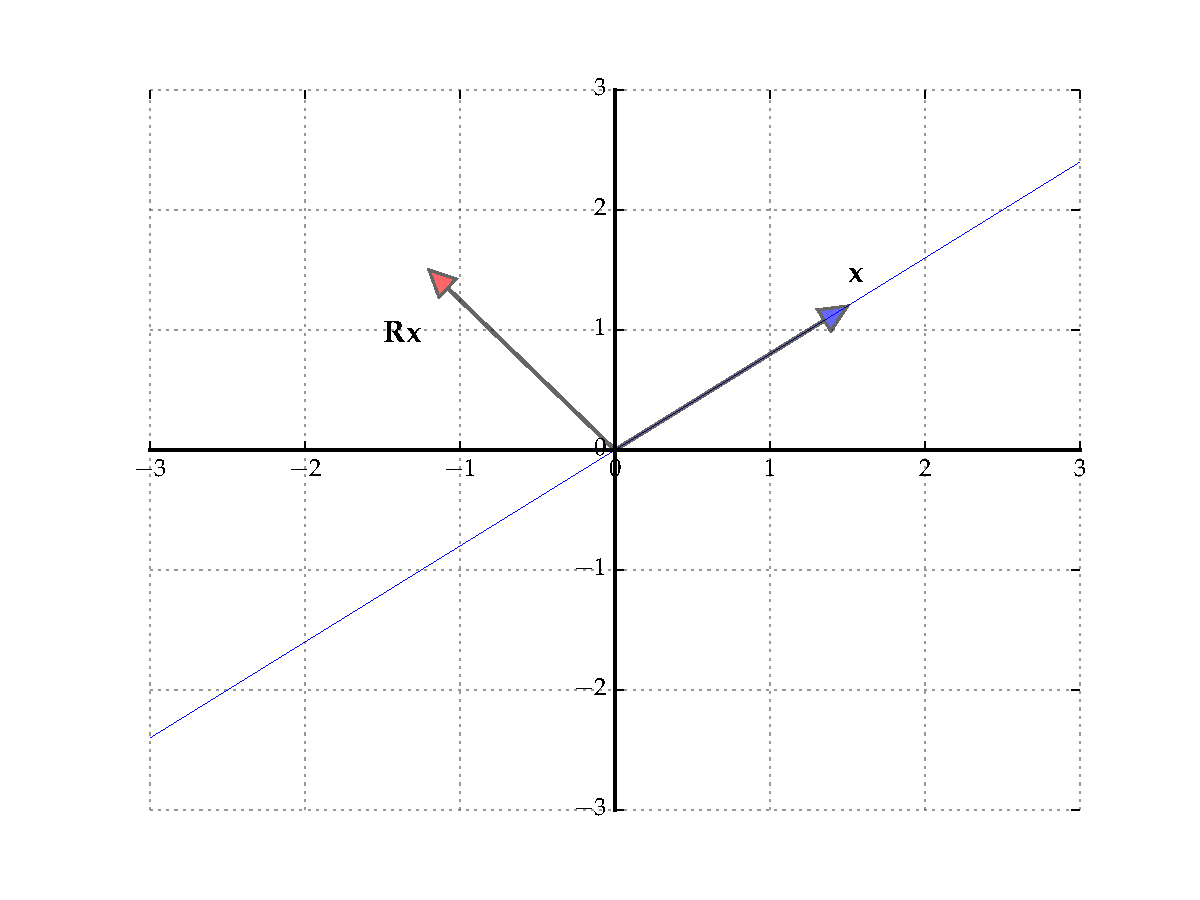
\includegraphics{rotation_1.pdf}}
        \caption{The matrix $\boldR$ rotates points by $90^{\circ}$}
       \end{center}
    \end{figure}

\end{frame}


\begin{frame}
    \
    \vspace{2em}
    \begin{figure}
       \begin{center}
        \scalebox{.4}{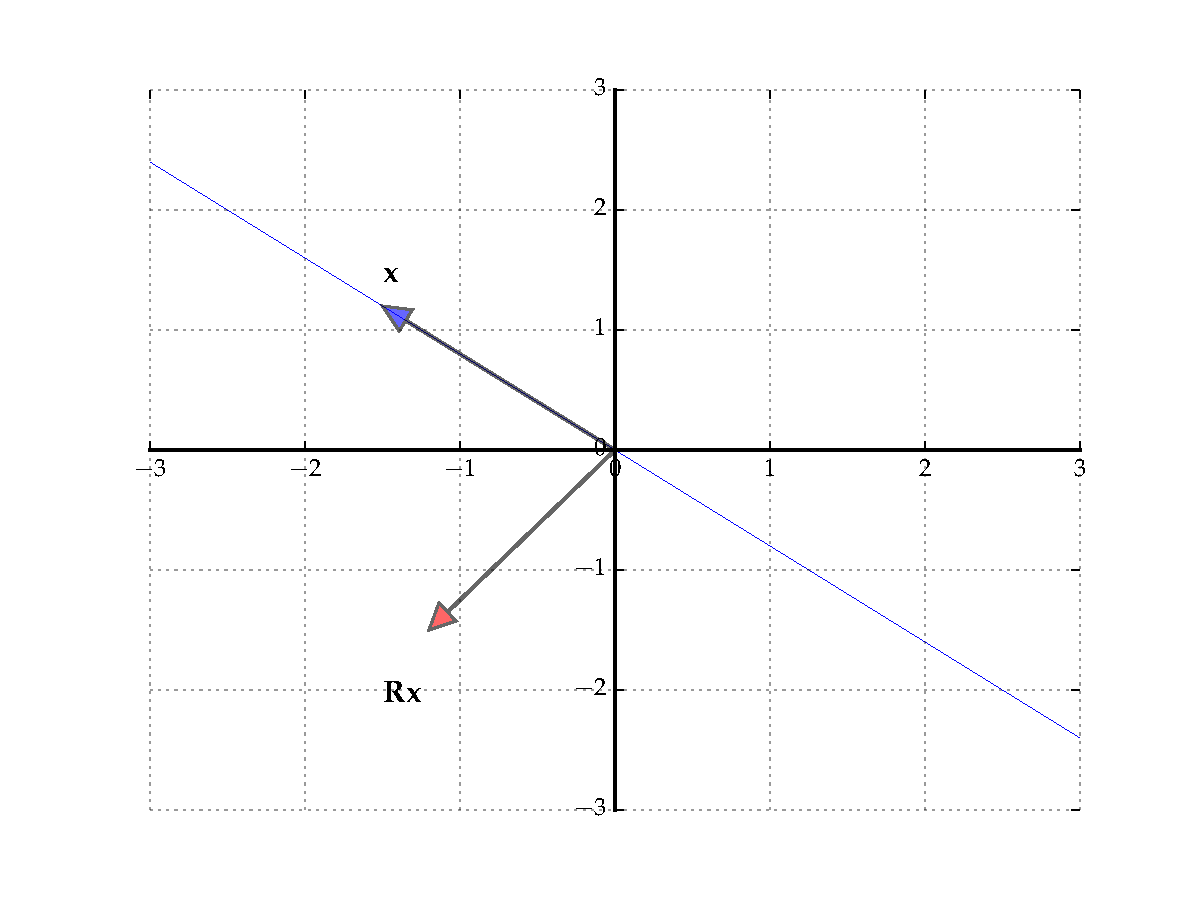
\includegraphics{rotation_2.pdf}}
        \caption{The matrix $\boldR$ rotates points by $90^{\circ}$}
       \end{center}
    \end{figure}

\end{frame}

\begin{frame}
    
    \vspace{2em}
    But $\boldR \boldx = \lambda \boldx$ can hold \underline{if} we allow
    complex values

    \vspace{1em}

    \Eg 
    %
    \begin{equation*}
        \left(
        \begin{array}{cc}
            0 & -1  \\
            1 & 0  \\
        \end{array}
        \right)
        \begin{pmatrix}
            1 \\
            -i
        \end{pmatrix}
        =
        \begin{pmatrix}
            i \\
            1
        \end{pmatrix}
        =
        i
        \begin{pmatrix}
            1 \\
            -i
        \end{pmatrix}
    \end{equation*}

    \vspace{.7em}
    That is,
    %
    \begin{equation*}
        \boldR \boldx = \lambda \boldx
        \quad \text{for} \quad
        \lambda := i
        \quad \text{and} \quad
        \boldx := 
        \begin{pmatrix}
            1 \\
            -i
        \end{pmatrix}
    \end{equation*}


    Hence $(\boldx, \lambda)$ is an eigenpair provided 
    we admit complex values 

\end{frame}

\begin{frame}
    
    \vspace{2em}
    \Fact{\eqref{ET-fa:chei}} For any square matrix $\boldA$ 
    %
    \begin{equation*}
        \lambda \text{ is an eigenvalue of } \boldA \; \iff \;
        \det(\boldA - \lambda \boldI) = 0
    \end{equation*}
    %

    \vspace{1em}

    \Prf  Let $\boldA$ by $N \times N$ and let $\boldI$ be the $N \times N$
    identity

    We have
    %
    \begin{align*}
        \det(\boldA - \lambda \boldI) = 0
        & \iff \boldA - \lambda \boldI \text{ is singular}
        \\
        & \iff \exists \, \boldx \not= \boldzero \st
            (\boldA - \lambda \boldI) \boldx = \boldzero
        \\
        & \iff \exists \, \boldx \not= \boldzero \st
        \boldA \boldx = \lambda \boldx
        \\
        & \iff \lambda 
        \text{ is an eigenvalue of } \boldA
    \end{align*}

\end{frame}

\begin{frame}
    
    \vspace{2em}
    \Eg In the $2 \times 2$ case,
    %
    \begin{equation*}
        \boldA =
        \left(
        \begin{array}{cc}
            a & b  \\
            c & d  \\
        \end{array}
        \right)
        \quad \implies \quad
        \boldA - \lambda \boldI =
        \left(
        \begin{array}{cc}
            a - \lambda & b  \\
            c & d - \lambda 
        \end{array}
        \right)
    \end{equation*}
    %
    \begin{align*}
        \fore
    \det(\boldA - \lambda \boldI) 
    & = (a - \lambda)(d - \lambda) - bc
    \\
    & = \lambda^2 - (a + d) \lambda + (ad - bc)
    \end{align*}
    
    Hence the eigenvalues of $\boldA$ are given by the two roots of 
    %
    \begin{equation*}
        \lambda^2 - (a + d) \lambda + (ad - bc) = 0
    \end{equation*}
    
    \vspace{.7em}
    Equivalently,
    %
    \begin{equation*}
        \lambda^2 - \trace(\boldA) \lambda + \det(\boldA) = 0
    \end{equation*}
    
\end{frame}


\begin{frame}

    \frametitle{Existence of Eigenvalues}

    \vspace{2em}
    Fix $N \times N$ matrix $\boldA$ 

    \vspace{0.5em}
    
    \Fact There exist complex numbers $\lambda_1, \ldots, \lambda_N$ such that
    %
    \begin{equation*}
        \det(\boldA - \lambda \boldI) = \prod_{n=1}^N (\lambda_n - \lambda)
    \end{equation*}
    %

    Each such $\lambda_i$  is an eigenvalue of $\boldA$ because
    %
    \begin{equation*}
        \det(\boldA - \lambda_i \boldI) 
        = \prod_{n=1}^N (\lambda_n - \lambda_i) 
        = 0
    \end{equation*}
    %
    
    Important: not all eigenvalues are necessarily distinct --- there can be repeats

\end{frame}

\begin{frame}

     \vspace{2em}
    \Fact{\eqref{ET-fa:eiprop}} 
    %
    Given $N \times N$ matrix $\boldA$ with eigenvalues $\lambda_1, \ldots, \lambda_N$
    we have
    %
    \begin{enumerate}
            \vspace{-0.6em}
        \item $\det(\boldA) = \prod_{n=1}^N \lambda_n$
            \vspace{0.4em}
        \item $\trace(\boldA) = \sum_{n=1}^N \lambda_n$
            \vspace{0.4em}
        \item If $\boldA$ is symmetric, then $\lambda_n \in \RR$ for all $n$
            \vspace{0.4em}
        \item If $\boldA$ is nonsingular, then $\text{eigenvalues of } \boldA^{-1}
                = 1/\lambda_1, \ldots, 1/\lambda_N$
            \vspace{0.4em}
        \item If $\boldA = \diag(d_1, \ldots, d_N)$, then $\lambda_n = d_n$ for all $n$
    \end{enumerate}

    \vspace{0.8em}
    %
    Hence $\boldA$ is nonsingular $\iff$ all eigenvalues are nonzero 
    
\end{frame}


\begin{frame}\frametitle{Quadratic Forms}

     \vspace{2em}
    Fix $N \times N$ matrix $\boldA$
    
    The \navy{quadratic
    function} or \navy{quadratic form} on $\RR^N$ associated with $\boldA$ is the
    map $Q$ defined by
    %
    \begin{equation*}
        Q(\boldx) := \boldx^\T \boldA \boldx = \sum_{j=1}^N \sum_{i=1}^N a_{ij} x_i x_j
    \end{equation*}
    
    \vspace{.7em}
    \Eg Let $N = 2$ and let $\boldA$ be the identity
    matrix $\boldI$.  In this case, 
    %
    \begin{equation*}
        Q(\boldx) = \| \boldx \|^2 = x_1^2 + x_2^2
    \end{equation*}
    
\end{frame}

\begin{frame}
    
    \vspace{2em}
    \begin{figure}
   \begin{center}
    \scalebox{.45}{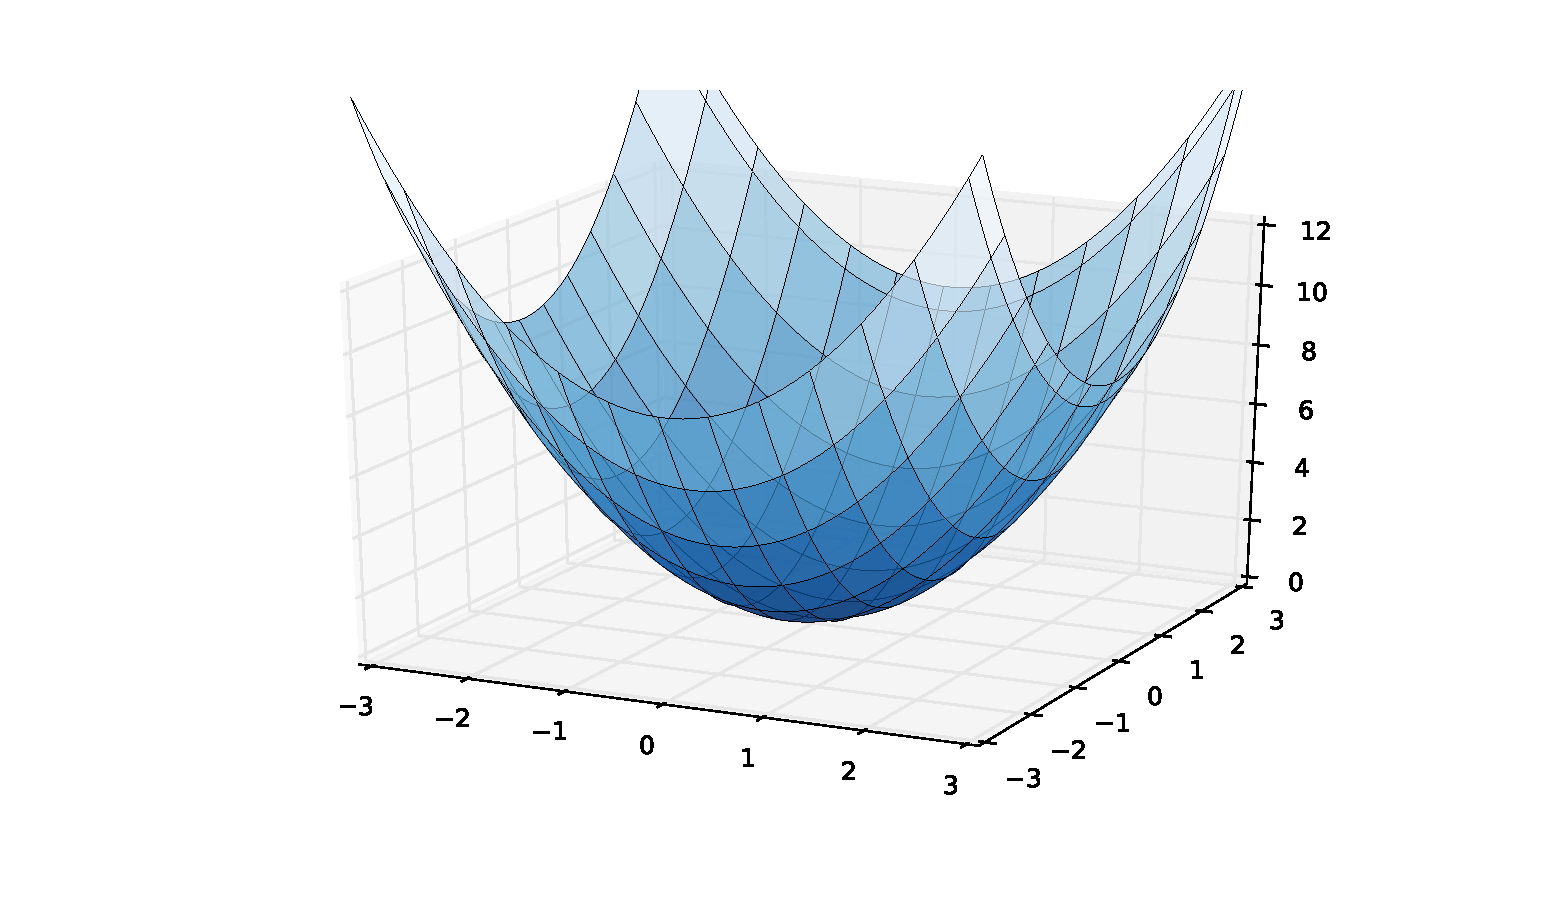
\includegraphics[trim={7.5em 2em 0 0em}, clip]{qform_pd.pdf}}
    \caption{\label{f:qform_pd} Quadratic function $Q(\boldx) = x_1^2 + x_2^2$ }
   \end{center}
    \end{figure}

\end{frame}

\begin{frame}

    \vspace{2em}
    Notice:
    \begin{itemize}
        \item The graph for $Q(\boldx) = \| \boldx \|^2 = x_1^2 + x_2^2$ lies everywhere above zero
    \end{itemize}
    
    \vspace{.7em}
    Matrix $\boldA$ with Quadratic form with the above property $Q(\boldx) \geq 0$  is called \emph{positive definite}
    
\end{frame}

\begin{frame}

    \vspace{2em}
    More generally, an $N \times N$ symmetric matrix $\boldA$ is called
    %
    \begin{itemize}
        \item \navy{nonnegative definite} if $\boldx^\T \boldA \boldx \geq 0$
            for all $\boldx \in \RR^N$, 
        \item \navy{positive definite} if $\boldx^\T \boldA \boldx > 0$ for all $\boldx
            \in \RR^N$ with $\boldx \not= \boldzero$,
        \item \navy{nonpositive definite} if $\boldx^\T \boldA \boldx \leq 0$
            for all $\boldx \in \RR^N$, and
        \item \navy{negative definite} if $\boldx^\T \boldA \boldx < 0$ for all $\boldx
            \in \RR^N$ with $\boldx \not= \boldzero$.
    \end{itemize}
    
    \vspace{.7em}
    If $\boldA$ fits none of these categories, then $\boldA$ is called \navy{indefinite}
    
\end{frame}

\begin{frame}

     \vspace{2em}
    \begin{figure}
   \begin{center}
    \scalebox{.45}{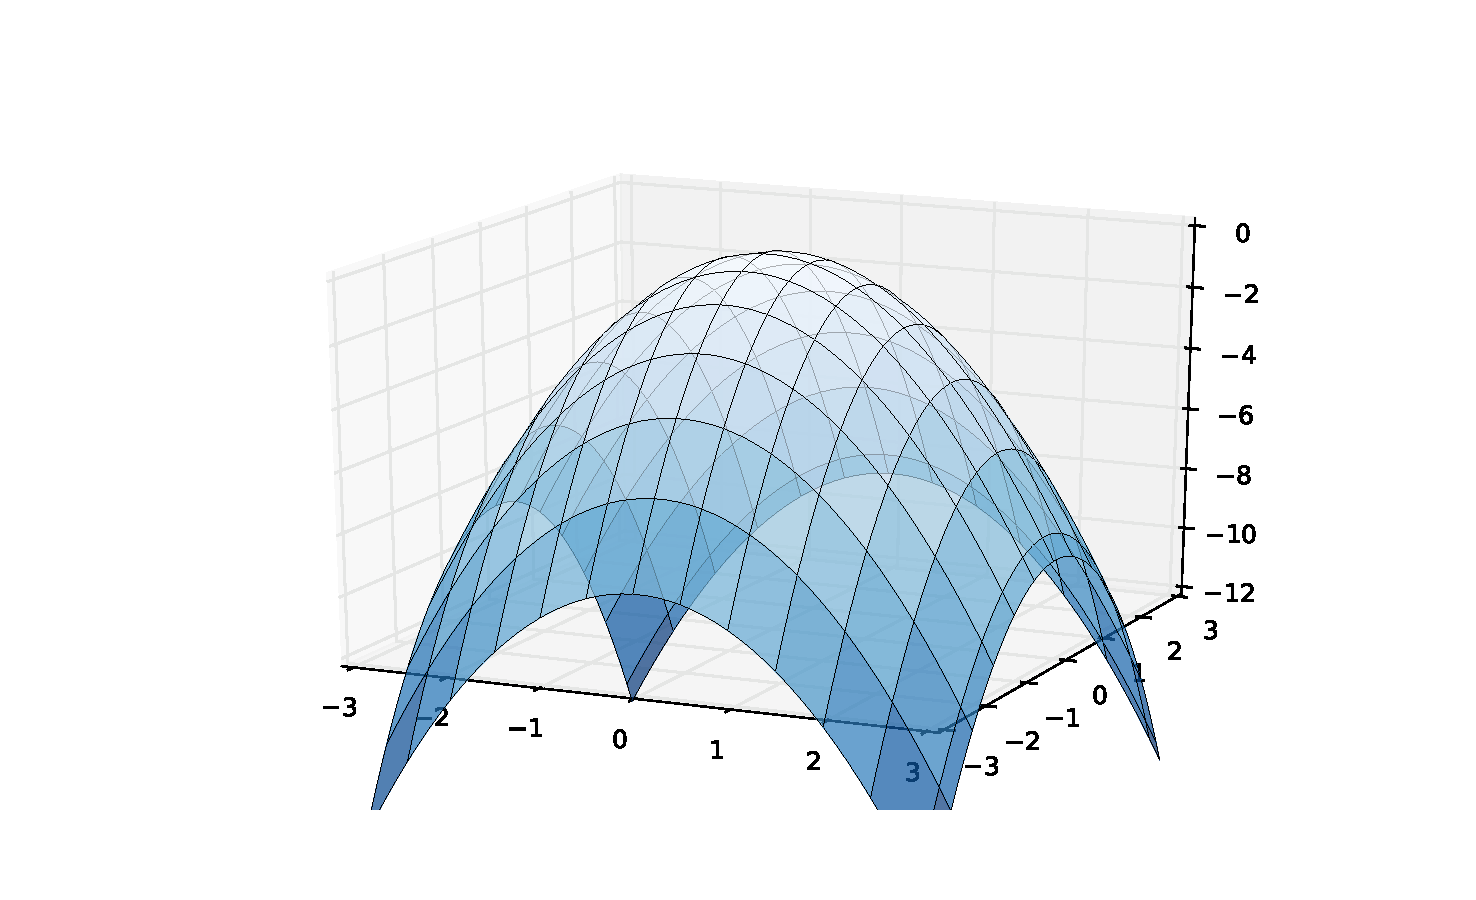
\includegraphics[trim={5em 2em 0 2em}, clip]{qform_nd.pdf}}
    \caption{\label{f:qform_nd} Quadratic function $Q(\boldx) = -x_1^2 - x_2^2$ }
   \end{center}
    \end{figure}
    
\end{frame}

\begin{frame}

     \vspace{2em}
    \begin{figure}
   \begin{center}
    \scalebox{.4}{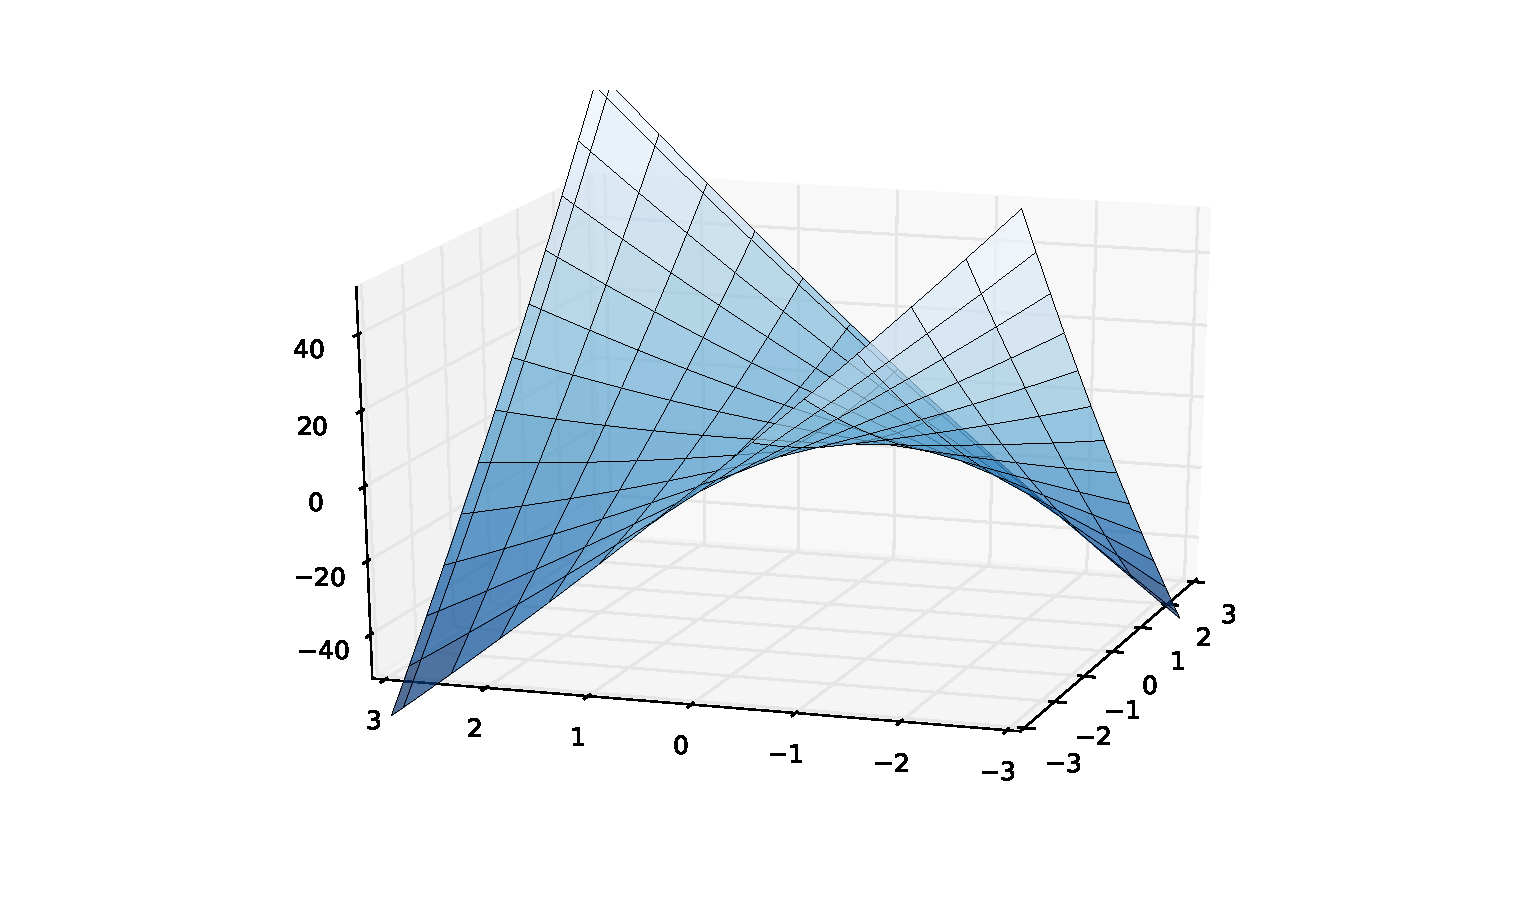
\includegraphics[trim={5em 2em 2em 2em}, clip]{qform_indef.pdf}}
    \caption{\label{f:qform_indef} Quadratic function $Q(\boldx) = x_1^2/2 +
        8 x_1 x_2 + x_2^2/2$ }
   \end{center}
    \end{figure}
    
\end{frame}

\begin{frame}  

   \vspace{2em}
   When the matrix $\boldA$ is diagonal: 
    %   
    \begin{equation*}
        \boldA = \diag(d_1, \ldots, d_N)
        \quad \text{implies} \quad
        Q(\boldx) = d_1 x_1^2 + \cdots + d_N x_N^2  
    \end{equation*}
    
    
    \vspace{.7em}
    A diagonal matrix is positive definite if and only if all diagonal elements are positive 
    
\end{frame}

\begin{frame}

    \vspace{2em}
    \Fact{\eqref{ET-fa:eigdef}}
    Let $\boldA$ be any symmetric matrix.  $\boldA$ is 
    %
    \begin{enumerate}
        \item positive definite if and only if its eigenvalues are all positive,
        \item negative definite if and only if its eigenvalues are all negative,
    \end{enumerate}
    %
    ...and similarly for nonpositive and nonnegative definite
    
    \vspace{.7em}
    \Fact{\eqref{ET-fa:ipde}}
        If $\boldA$ is positive definite, then $\boldA$ is nonsingular, with $\det \boldA > 0$

\end{frame}

\begin{frame}

     \vspace{2em}
    A necessary (but not sufficient) condition for each kind of definiteness:
    
    \vspace{.7em}
    \Fact{\eqref{ET-fa:ipde0}}
        If $\boldA$ is positive definite, then
        each element $a_{nn}$ on the principal diagonal is positive, and the same
        for nonnegative, nonpositive and negative.
        
\end{frame}

\section{Projection and Decomposition}

\begin{frame}\frametitle{Projection Matrices}

     \vspace{2em}
    Recall given any subspace of $\mathbb{R}^{N}$, $S$, the corresponding
    projection $\boldP = \proj S$ is a linear map from $\RR^N$ to $\RR^N$

    \vspace{.7em}
    Recall Theorem~\ref{ET-t:lmaeq}: there exists an $N \times N$ matrix $\hat \boldP$ such that $\boldP \boldx =
    \hat \boldP \boldx$ for all $\boldx \in \RR^N$
    %
    \begin{itemize}
        \item from now on $\boldP$ will also represent
    the corresponding matrix
    \end{itemize} 
    
    What does this matrix look like?
    
\end{frame}

\begin{frame}

     \vspace{.7em}
    \Thm {\eqref{ET-t:projon}}
    Let $S$ be a subspace of $\RR^N$.  If $\boldP = \proj S$, then
    %
    \begin{equation}
        \label{eq:projb}
        \boldP = \boldB (\boldB^\T\boldB)^{-1} \boldB^\T  
    \end{equation}
    %
    for every matrix $\boldB$ such that the columns of $\boldB$ form a basis
    of $S$ 
    
    \vspace{.7em}
    See exercise~\ref{ET-ex:projon} for proof
    
    \begin{itemize}
        \item  The matrix $\boldM = \boldI -
                \boldP$ denotes the residual projection (see page~\pageref{ET-eq:ann0})
    \end{itemize}
    
\end{frame}

\begin{frame}
    
    \vspace{2em}
    \Eg
    Recall example~\ref{ET-eg:pvones} on page~\pageref{ET-eg:pvones}
    
    We found the projection of $\boldy \in \RR^N$ onto $\Span\{\boldone\}$ is
    $\bar y \boldone$
    
    Same result using Theorem~\eqref{ET-t:projon}:
    \begin{itemize}
        \item Since $\boldone$ is a basis for $\Span\{\boldone\}$:
            %
            \begin{equation*}
                \label{eq:pcz}
                \boldP = \proj \; \Span\{\boldone\} 
                \; \implies \;
                \boldP 
                = \boldone (\boldone^\T\boldone)^{-1} \boldone^\T  
                = \frac{1}{N} \boldone \boldone^\T  
            \end{equation*}
        %
        \item Thus, $\boldP \boldy = \bar y \boldone$, as expected
        \item Corresponding residual projection is
        %
        \begin{equation*}
            \label{eq:pczm}
            \boldM_c
            = \boldI - \frac{1}{N} \boldone \boldone^\T  
        \end{equation*}
    \end{itemize}

\end{frame}

\begin{frame}

     \vspace{2em}
    \Fact{\eqref{ET-fa:anox}} 
    In the setting of theorem~\ref{ET-t:projon}, we have 
    %
    \begin{enumerate}
        \item $\boldM \boldB = \boldzero$
        \item $\boldP \boldB = \boldB$
    \end{enumerate}
    
    Proof is an exercise (ex. \ref{ET-ex:anox} in ET)
    
    \vspace{1em}
    Easy to see $\boldM_c$ in the previous example maps
    $\boldone$ to $\boldzero$
    
\end{frame}

\begin{frame}
    
    \vspace{2em}
    A square matrix $\boldA$ is \navy{idempotent} if $\boldA \boldA = \boldA$ 
    
    \vspace{.7em}
    \Fact{\eqref{ET-fa:pmsi}}
        Both $\boldP$ and $\boldM$ are symmetric and idempotent
    
    (Exercise: check by direct calculation)
    
    \vspace{.7em}
    Intuition: projecting
    onto a subspace twice is the same as projecting once -- recall fact~\ref{ET-fa:opt3} on page~\pageref{ET-fa:opt3}
    
\end{frame}

\begin{frame}
    
    \vspace{2em}
    \Fact{\eqref{ET-fa:trop}}
    Let $S$ be a linear subspace of $\RR^N$. If $\boldP = \proj S$ and 
    $\boldM$ is the residual projection, then 
    %
    \begin{enumerate}
        \item $\rank \boldP  = \trace \boldP  = \dim S$ and
        \item $\rank \boldM  = \trace \boldM  = N - \dim S$
    \end{enumerate}
  
  
    \Prf
    \begin{itemize}
        \item The rank of a linear
            map is the dimension of its range.  When $\boldP = \proj S$, the range of
            $\boldP$ is exactly $S$
        \item To show that $\trace \boldP = \dim S$ also holds, use
                fact~\ref{ET-fa:idtrra}--  $\trace\boldP
                = \dim S$, 
        \item It follows that $\trace\boldM = N - \dim S$, because
            %
            \begin{equation*}
                \trace\boldM 
                = \trace(\boldI - \boldP) 
                = \trace \boldI - \trace\boldP 
                = N - \dim S
            \end{equation*}

    \end{itemize}
  
\end{frame}


\begin{frame}\frametitle{Overdetermined Systems of Equations}
    
    \vspace{2em}
    Consider systems of
    equations of the form $\boldA \boldx = \boldb$ when:
    \begin{itemize}
        \item The matrix $\boldA$ is
        $N \times K$ and has full column rank
        \item The vector $\boldx$ is $K\times1$
        \item The vector $\boldb$ is $N\times 1$ 
        \item $K\leq N$
    \end{itemize} 
    
    \vspace{1em}
    Taking $\boldA$ and $\boldb$ as given, we seek $\boldx \in \RR^K$ such that
    $\boldA \boldx = \boldb$

\end{frame}

\begin{frame}

     \vspace{2em}
    If $K = N$, then system has precisely one solution
    
    \vspace{1em}
    When $N > K$, the system of equations said to be \navy{overdetermined}:
    %
    \begin{itemize}
        \item number of equations $>$ number of unknowns
        \item number of constraints $>$ degrees of freedom
    \end{itemize}
    
    May not be able find a $\boldb$ that satisfies all $N$ equations  
    
\end{frame}

\begin{frame}

     \vspace{2em}
    Recall  the linear map $T \colon
    \RR^K \to \RR^N$ corresponding to $\boldA$ is $T\boldx = \boldA \boldx$
    
    \vspace{1em}
    The following statements are equivalent:
    %
    \begin{enumerate}
        \item there exists an $\boldx \in \RR^K$ with $\boldA \boldx = \boldb$
        \item the vector $\boldb \in \colspace \boldA$
        \item the vector $\boldb \in \range T$
    \end{enumerate}
    
     \vspace{.7em}
    Theorem~\ref{ET-t:lfoc} on page~\pageref{ET-t:lfoc}: when $K <
    N$, the function $T$ cannot be onto -- possible $\boldb$ lies 
    outside the range of $T$
    
\end{frame}

\begin{frame}

     \vspace{2em}
    When $K < N$, the scenario $\boldb \in
    \colspace \boldA$ is ``very rare" because:
    %
    \begin{itemize}
        \item the point $\boldb$ is an arbitrary point in $\RR^N$
        \item the space $ \colspace \boldA$ has dimension $K$
        \item $K$-dimensional subspaces of $\RR^N$ have 
        ``Lebesgue measure zero'' -- the ``chance'' of $\boldb$ happening to lie in this subspace is tiny  
    \end{itemize}
    
\end{frame}

\begin{frame}

     \vspace{2em}
    Standard approach: admit an exact solution may not
    exist
    
    \vspace{1em}
    Focus on finding $\boldx \in \RR^K$ to make $\boldA
    \boldx$ as close to $\boldb$ as possible
    \begin{itemize}
        \item close in terms of ordinary Euclidean norm
    \end{itemize}
    
    \vspace{1em}
    The minimization problem, called the \navy{least squares problem}
    %
    \begin{equation}
        \label{eq:mxls}
        \hat{\boldx} \colon = \argmin_{\boldx \in \RR^K} \| \boldb - \boldA \boldx \|
    \end{equation}
    
\end{frame}


\begin{frame}

     \vspace{2em}
    Assuming $\boldA$ is $N \times K$ with $K \leq N$ and $\boldb$ is $N \times 1$, 
    we can use  the orthogonal projection theorem to solve \eqref{eq:mxls}
    
    \vspace{.7em}
    \Thm{\eqref{ET-t:lssol}}
        If $\boldA$ has full column rank, then \eqref{eq:mxls} has the unique
        solution
        %
        \begin{equation}
            \label{eq:dlse}
            \hboldx := (\boldA^\T \boldA)^{-1} \boldA^\T \boldb
        \end{equation}
        %
    \end{frame}
    
\begin{frame}

    \vspace{2em}
    \Prf 
    
    Let:
    %
    \begin{itemize}
        \item $\boldA$ and $\boldb$ be as in the statement of the theorem
        \item $\hboldx$ be as in \eqref{eq:dlse} and
        \item $S := \colspace \boldA$
    \end{itemize}
    %
    By full column rank assumption, the columns of $\boldA$ form a basis for
    $S$. Applying theorem~\ref{ET-t:projon}, orthogonal projection of $\boldb$
    onto $S$ is 
    %
    \begin{equation}
        \label{eq:ibprojon}
        \boldP\boldb 
        := \boldA (\boldA^\T \boldA)^{-1} \boldA^\T \boldb  
         = \boldA \hboldx
    \end{equation}
    
    Since the orthogonal projection theorem gives a unique
    minimizer in terms of the closest point in $S$ to $\boldb$,
    %
    \begin{equation}
        \label{eq:sfy}
        \| \boldb - \boldA\hboldx \| < \| \boldb - \boldy\|
        \quad \text{for all } \boldy \in S, \; \boldy \not= \boldA \hboldx
    \end{equation}

\end{frame}
    
\begin{frame}
    
    \vspace{2em}
    \Prf (cont.) Pick any $\boldx \in \RR^K$ such that $\boldx \not= \hboldx$
    
    We have $\boldA \boldx \in S$
    
    In addition, since $\boldx \not= \hboldx$, and since $\boldA$ has full column
    rank, it must be that $\boldA \boldx \not= \boldA \hboldx$
    (ex.~\ref{ET-ex:ui})
    
     \vspace{.7em}
    Hence
    %
    \begin{equation*}
        \| \boldb - \boldA\hboldx \| < \| \boldb - \boldA \boldx\|
        \quad \text{for all } \boldx \in \RR^K, \; \boldx \not= \hboldx
    \end{equation*}
    %
    In other words, $\hboldx$ is the unique solution to \eqref{eq:mxls}
    
\end{frame}

\begin{frame}

    \vspace{2em}
    In  \eqref{eq:dlse}, the matrix $(\boldA^\T\boldA)^{-1} \boldA^\T$ 
    is called the \navy{pseudoinverse} of $\boldA$ 
    
    \vspace{1em}
    If $K =
    N$, then the
    least squares solution $\hboldx$ in \eqref{eq:dlse} reduces to:
    %
    \begin{equation*}
        \boldx = \boldA^{-1}\boldb
    \end{equation*}
    
\end{frame}

\begin{frame}

     \vspace{2em}
    What happens if the columns of $\boldA$ are not
    linearly independent? 
    
    \begin{itemize}
        \item   the set $\colspace \boldA$ is still a linear
        subspace and the orthogonal projection theorem still gives us a closest
        point $\boldP \boldb$ to $\boldb$ in $\colspace \boldA$
        \item   since $\boldP
        \boldb \in \colspace \boldA$, there still exists a vector $\hboldx$ such
        that $\boldP \boldb = \boldA \hboldx$
        \item    but there
        exists an infinity of such vectors
    \end{itemize}
    
    See Exercise~\ref{ET-ex:lsiosol}
    
\end{frame}


\section{Diagonalisation and Spectral Theory} 

\begin{frame}\frametitle{QR Decomposition}

     \vspace{2em}
    The \navy{QR decomposition} of a given matrix $\boldA$ is a product of the form $\boldQ \boldR$
    \begin{itemize}
        \item first matrix has orthonormal columns and 
        \item the second is upper triangular
    \end{itemize}
    
    \vspace{1em}
    Applications include least squares problems and the computation of eigenvalues
    
\end{frame}

\begin{frame}

     \vspace{2em}
    \Thm{\eqref{ET-t:qr}}
    If $\boldA$ is an $N \times K$ matrix with full column rank, then there exists a
    factorization $\boldA = \boldQ \boldR$ where
    %
    \begin{enumerate}
        \item $\boldR$ is $K \times K$, upper triangular and nonsingular, and 
        \item $\boldQ$ is $N \times K$, with orthonormal columns
    \end{enumerate}
    %
    See page~\pageref{ET-t:qr} in ET for a proof
    
\end{frame}

\begin{frame}

     \vspace{2em}
    Given the decomposition $\boldA = \boldQ \boldR$, the least squares solution
    $\hboldx$ defined in \eqref{eq:dlse} can also be written as:
    $$\hboldx =
    \boldR^{-1} \boldQ^\T \boldb$$
    
    See Ex.~\ref{ET-ex:qrlsq}
    
    \vspace{.7em}
    Premultiplying by $\boldR$:
    $$\boldR \hboldx = \boldQ^\T \boldb$$
    
\end{frame}

\begin{frame}\frametitle{Diagonalisation and Spectral Theory}

     \vspace{2em}
    If $f \colon A \to A$ and $g \colon B \to B$, then
    $g$ is said to be \navy{topologically conjugate} to $f$ whenever there exists
    a continuous bijection $\tau \colon B \to A$ such that $$f = \tau \circ g \circ
    \tau^{-1}$$
    
    \vspace{.7em}
    Can be beneficial if $g$ is somehow simpler
    than $f$
    
\end{frame}

\begin{frame}

    \vspace{2em}
    A square matrix $\boldA$ is said to be \navy{similar} to another matrix $\boldB$ if there exists an invertible matrix $\boldP$ such that $\boldA = \boldP \boldB \boldP^{-1}$

    \begin{figure}
   \begin{center}
    \begin{tikzpicture}[scale=1,
    axis/.style={->, >=stealth'},
    important line/.style={thick},
    dashed line/.style={dashed, thin},
    every node/.style={color=black},
    decoration={brace,amplitude=7pt},
    ] 

%% draw nodes
\coordinate (x1) at (-2,2);  \coordinate (x11) at (-2,1.8); \coordinate (x12) at (-1.8,2);  
\coordinate (x2) at (-2,0); \coordinate (x21) at (-1.8,0); \coordinate (x22) at (-2,0.2);
\coordinate (x3) at (2,2);   \coordinate (x31) at (1.8,2);  \coordinate (x32) at (2,1.8);
\coordinate (x4) at (2,0);  \coordinate (x41) at (1.8,0); \coordinate (x42) at (2,0.2);

\node[fill=black,circle,scale=0.37] at (x1){};
\node[fill=black,circle,scale=0.37] at (x2){};
\node[fill=black,circle,scale=0.37] at (x3){};
\node[fill=black,circle,scale=0.37] at (x4){};

%% label x & Ax
\draw (x2) node[below=5pt] {$\boldx$};
\draw (x4) node[below=5pt] {$\boldA\boldx$};

%% draw arrows
\draw[important line, ->]  (x21) -- node[above=5pt] {$\boldA$} (x41);
\draw[important line, ->]  (x22) -- node[left=5pt] {$\boldP^{-1}$} (x11);
\draw[important line, ->]  (x12) -- node[above=5pt] {$\boldB$} (x31);
\draw[important line, ->]  (x32) -- node[right=5pt] {$\boldP$} (x42);
  
\end{tikzpicture}

    \caption{\label{f:diagonalize} $\boldA$ is similar to $\boldB$}
   \end{center}
    \end{figure}
    
\end{frame}

\begin{frame}
   
    \vspace{2em}
    If $\boldA$ is similar to a diagonal matrix, then $\boldA$ is
    called \navy{diagonalizable}
    
    \vspace{.7em}
    We are interested in similarity to simple matrices, and diagonal matrices are the simplest kind 
    
\end{frame}

\begin{frame}

     \vspace{2em}
    \Fact{\eqref{ET-fa:powsm}}
        If $\boldA$ is similar to $\boldB$, then $\boldA^t$ is similar to
        $\boldB^t$ for all $t \in \NN$
    
    \vspace{.7em}
    \Eg
    We want to calculate $\boldA^t$ for some given $t \in \NN$ 
    
    If $\boldA = \boldP \boldLambda \boldP^{-1}$ for some
    $\boldLambda = \diag(\lambda_1, \ldots, \lambda_N)$, then by
    fact~\ref{ET-fa:powsm} and fact~\ref{ET-fa:powdm}, we
    have
    %
        $$\boldA^t = \boldP \diag(\lambda_1^t, \ldots, \lambda_N^t)
        \boldP^{-1}$$
    
\end{frame}

\begin{frame}\frametitle{Diagonalization and Eigenvalues}

    \vspace{.7em}
    \Fact{\eqref{ET-fa:diagee}}
    If $\boldA = \boldP \boldLambda \boldP^{-1}$ for some $\boldLambda =
        \diag(\lambda_1, \ldots, \lambda_N)$, then $(\col_n \boldP,
            \lambda_n)$ is an eigenpair of $\boldA$ for each $n$
            
    \vspace{.7em}    
    
    \Prf
    Observe $\boldA
    = \boldP \boldLambda \boldP^{-1}$ implies $\boldA \boldP = \boldP \boldLambda$
    
    Equating the $n$th column on each side gives 
    %
        $$\boldA \boldp_n = \lambda_n
        \boldp_n$$
    %
    Where $\boldp_n := \col_n \boldP$
    
    Note  $\boldp_n$ is not the
    zero vector because $\boldP$ is invertible
        
\end{frame}

\begin{frame}
    
    \vspace{2em}
    But when is $\boldA$ diagonalizable?  
    
    \vspace{.7em}
    \Fact (3.3.7)
    An $N \times N$ matrix $\boldA$ is diagonalizable if and only if
    it has $N$ linearly independent eigenvectors

\end{frame}


\begin{frame}

     \vspace{2em}
    In some cases, we can get an even simpler matrix decomposition if 
    the matrix $\boldP$ has orthogonal columns 

    These kinds of matrices are called \navy{orthogonal matrices}
    
    \vspace{.7em}
    \Fact{\eqref{ET-fa:orthmat}}
    If $\boldQ$ and $\boldP$ are $N \times N$ orthogonal matrices, then
    %
    \begin{enumerate}
        \item $\boldQ^\T$ is orthogonal and $\boldQ^{-1} = \boldQ^\T$,
        \item $\boldQ \boldP$ is orthogonal, and
        \item $\det \boldQ \in \{-1, 1\}$.
    \end{enumerate}
    
\end{frame}
    
\begin{frame}

    \vspace{2em}
    If $\boldA = \boldQ \boldLambda \boldQ^{-1}$ and $\boldQ$ has orthonormal columns,
    then $$\boldA = \boldQ \boldLambda \boldQ^\T$$
    
    Clearly, $\boldA$ must be symmetric. Next theorem shows symmetry of $\boldA$ is also sufficient
    
    \vspace{.7em}
    \Thm{\eqref{ET-t:dismat}}
    If $\boldA$ is symmetric, then $\boldA$ can be
    diagonalized as $\boldA = \boldQ \boldLambda \boldQ^\T$, where 
    $\boldQ$ is an orthogonal matrix and $\boldLambda$ is the 
    diagonal matrix formed from the eigenvalues of $\boldA$
    
\end{frame}

\begin{frame}

   \vspace{2em}

    Above theorem was a version of the \navy{spectral decomposition theorem}

    $\boldQ \boldLambda \boldQ^\T$ is called the \navy{symmetric eigenvalue
    decomposition} of $\boldA$\ -- action of $\boldA$ on an
    $N \times 1$ vector $\boldx$:
    %
    \begin{equation*}
        \boldA\boldx = \sum_{n=1}^N \lambda_n (\boldu_n^\T \boldx) \boldu_n
    \end{equation*}
    %
    where $\lambda_n$ is the $n$th eigenvalue of $\boldA$ and $\boldu_n = \col_n \boldQ$
    
    \vspace{.7em}
    Compare with $\boldx = \sum_{n=1}^N (\boldu_n^\T \boldx) \boldu_n$
    
\end{frame}

\begin{frame}

    \vspace{2em}
    \Fact{\eqref{ET-fa:sqrtsnd}}
    If $\boldA$ is nonnegative definite, then $\sqrt{\boldA}$
    exists and equals $\boldQ \sqrt{\boldLambda} \boldQ^\T$.
    The matrix $\sqrt{\boldLambda}$ is given by $\diag(\sqrt{\lambda_1},
    \ldots, \sqrt{\lambda_N})$
    
    \vspace{.7em}
    \Fact{\eqref{ET-fa:cholesky}}
    If $\boldA$ is positive definite, then there exists a nonsingular, upper
    triangular matrix $\boldR$ such that $\boldA = \boldR^\T \boldR$
    
    This decomposition is called the \navy{Cholesky decomposition}

\end{frame}

\begin{frame}

    \vspace{2em}
    \Prf (Cholesky decomposition)
    We can write:
    %
        \begin{equation*}
            \boldA 
            = \boldQ \boldLambda \boldQ^\T
            = \boldQ \sqrt{\boldLambda} \sqrt{ \boldLambda} \boldQ^\T
            = (\sqrt{ \boldLambda} \boldQ^\T)^\T \sqrt{ \boldLambda} \boldQ^\T
        \end{equation*}
    %
    Then apply the QR decomposition to $\sqrt{ \boldLambda} \boldQ^\T$:
    %
        $$\sqrt{ \boldLambda} \boldQ^\T = \tilde \boldQ \boldR$$
    %
    where $\boldR$ is nonsingular and upper triangular, and $\tilde \boldQ$ has
    orthonormal columns
    
    \vspace{.7em}
    Because the columns of $\tilde \boldQ$ are orthonormal,
    %
        \begin{equation*}
        \boldA 
        = (\tilde \boldQ \boldR)^\T \tilde \boldQ \boldR
        =  \boldR^\T \tilde \boldQ^\T \tilde \boldQ \boldR
        =  \boldR^\T \boldR
        \end{equation*}
    
\end{frame}


\begin{frame}

    \vspace{2em}
    \frametitle{Norms and Continuity}
    
    Given vector sequence $\{\boldx_n\}$ in $\RR^K$ and any point $\boldx \in \RR^K$, we say that $\{\boldx_n\}$ \navy{converges} to $\boldx$ and write
    \navy{$\boldx_n \to \boldx$} if, for any $\epsilon > 0$, there exists an $N
    \in \NN$ such that $\|\boldx_n - \boldx\| < \epsilon$ whenever $n \geq N$
    
    \vspace{.7em}
    Equivalently, the real-valued sequence $z_n := \|\boldx_n - \boldx\|$
    converges to zero in $\RR$ as $n \to \infty$

\end{frame}

\begin{frame}
    
    \vspace{2em}
    \Fact (3.3.11)
    The following results hold:
    %
    \begin{enumerate}
        \item If $\boldx_n \to \boldx$ and $\boldy_n \to \boldy$, then $\boldx_n +
            \boldy_n \to \boldx +  \boldy$.
        \item If $\boldx_n \to \boldx$ and $\alpha \in \RR$, then $\alpha \boldx_n 
            \to \alpha \boldx$.
        \item $\boldx_n \to \boldx$ if and only if $\bolda^\T \boldx_n \to
            \bolda^\T \boldx$ for all $\bolda \in \RR^K$.
    \end{enumerate}


\end{frame}

\begin{frame}

    \vspace{2em}
    We want to extend notion of convergence to matrices
    
    \vspace{.7em}
    The \navy{matrix norm} of $N \times K$ matrix $\boldA$:
    %
    \begin{equation}
    \label{eq:mn}
    \| \boldA \| :=
    \max \left\{ 
        \| \boldA \boldx \| \,: \, 
        \boldx \in \RR^K, \; \| \boldx \| = 1
        \right\}
    \end{equation}

    \vspace{.7em}
    The value of the matrix norm is not easy to solve for in
    general
    
    However, the matrix
    norm behaves like the vector norm
    
\end{frame}

\begin{frame}

    \vspace{2em}
    \Fact (3.3.12)
    For any conformable matrices $\boldA$ and $\boldB$, the matrix norm 
    satisfies
    %
    \begin{enumerate}
        \item $\| \boldA \| \geq 0$ and $\| \boldA \| = 0$ if and only if all entries of
            $\boldA$ are zero,
        \item $\| \alpha \boldA \| = |\alpha| \| \boldA \|$ for any scalar
            $\alpha$,
        \item $\| \boldA + \boldB \| \leq \| \boldA \| + \| \boldB \|$, and
        \item $\| \boldA \boldB \| \leq \| \boldA \| \| \boldB \|$.
    \end{enumerate}
    
    
\end{frame}

\begin{frame}

    \vspace{2em}
    \Fact{\eqref{ET-fa:mnbd}}
    For any $J \times K$ matrix $\boldA$ with elements $a_{jk}$, we have
    %
    \begin{equation*}
        \| \boldA \| \leq \sqrt{JK} \max_{jk} |a_{jk}|
    \end{equation*}
    
    \vspace{1em}
    If every element of
    $\boldA$ is close to zero then $\| \boldA \|$ is also close to zero

\end{frame}

\begin{frame}\frametitle{Neumann Series}

    \vspace{2em}
    Later on, we study dynamic systems of the form
    %
        $$\boldx_{t+1} = \boldA \boldx_t + \boldb$$
    %
    
    \vspace{.7em}
    Does there exist a ``stationary" vector
  $\boldx \in \RR^N$, in the sense that $\boldx_t = \boldx$ implies $\boldx_{t+1} =
  \boldx$?
  
    We seek an $\boldx \in \RR^N$ that solves the
    system of equations
    %
    \begin{equation}
        \label{eq:lpfde}
        \boldx = \boldA \boldx + \boldb 
        \qquad (\boldA \text{ is } N \times N \text{ and } \boldb \text{ is } N
        \times 1)
    \end{equation}
    
\end{frame}

\begin{frame}
    
    \vspace{2em}
    Consider the scalar case $x = a x + b$
    
    \vspace{.7em}
    If $|a| < 1$, then there is a unique solution
    %
    \begin{equation*}
        \bar x 
        = \frac{b}{1-a} 
        = b \sum_{k=0}^{\infty} a^k 
    \end{equation*}
 
    \vspace{.7em}
    The Neumann series Lemma helps generalise to $\mathbb{R}^{N}$
    
    \vspace{1em}
    \Thm{\eqref{ET-t:nms}}
    If $\boldA$ is square and $\| \boldA^j \| < 1$
    for some $j \in \NN$, then $\boldI - \boldA$ is invertible, and
    %
    \begin{equation*}
        \label{eq:nmse}
        (\boldI - \boldA)^{-1} = \sum_{i=0}^{\infty} \boldA^i 
    \end{equation*}
    
\end{frame}
 
\begin{frame}

    \vspace{.7em}
    When the condition of the Neumann series lemma holds, \eqref{eq:lpfde}
    has the unique solution
    %
    \begin{equation*}
        \bar \boldx 
        = (\boldI - \boldA)^{-1} \boldb 
        = \sum_{i=0}^{\infty} \boldA^i  \boldb 
    \end{equation*}
    
    To test the condition, we use the  \navy{spectral radius} of
    $\boldA$:
    %
    \begin{equation*}
        \label{eq:srmn}
        \rho(\boldA) := \max \setntn{ |\lambda| }
        { \lambda \text{ is an eigenvalue of } \boldA}
    \end{equation*}
    
    \vspace{1em}
    $|\lambda|$ is the \navy{modulus} of the possibly complex number
    $\lambda$
    

\end{frame}

\begin{frame}

    \vspace{2em}
    \Fact
    If $\rho(\boldA) < 1$, then $\| \boldA^j \| < 1$ for some $j \in \NN$
    
    \vspace{.7em}
    Why is $\rho(\boldA) < 1$ is sufficient?
    
    We need
    $\sum_{i=0}^t \boldA^i (\boldI - \boldA)$ to close be $\boldI$ for
    large $t$
    
    We have:
    \begin{equation*}
        \sum_{i=0}^t \boldA^i (\boldI - \boldA)
        =
        \sum_{i=0}^t \boldA^i - \sum_{i=0}^t \boldA^{i+1}
        =
        \boldI - \boldA^{t+1}
    \end{equation*}

\end{frame}

\begin{frame}
    
    \vspace{2em}
    Simplify to the case where $\boldA$ is diagonalizable:
    %
        $$\boldA = \boldP \boldLambda \boldP^{-1}$$
    %
    where $\boldLambda$ is a diagonal
    matrix containing the eigenvalues $\lambda_1, \ldots, \lambda_N$ of $\boldA$
    on its principal diagonal

    \vspace{.7em}
    Now, use fact~\ref{ET-fa:powsm},
    %
    \begin{equation*}
        \boldA^t
        = \boldP
        \left(
        \begin{matrix}
            \lambda_1^t & 0 & \cdots & 0 \\
            0 & \lambda_2^t & \cdots & 0 \\
            \vdots & \vdots &  & \vdots \\
            0 & 0 & \cdots & \lambda_N^t \\
        \end{matrix}
        \right)
        \boldP^{-1}
    \end{equation*}
    %
    If $\rho(\boldA) < 1$, then $|\lambda_n| < 1$ for all $n$, and hence
    $\lambda_n^t \to 0$ as $t \to \infty$. It follows that $\boldA^t \to
    \boldzero$ 
    
\end{frame}


\end{document}

